\documentclass[14pt]{beamer}\usepackage[]{graphicx}\usepackage[]{color}
%% maxwidth is the original width if it is less than linewidth
%% otherwise use linewidth (to make sure the graphics do not exceed the margin)
\makeatletter
\def\maxwidth{ %
  \ifdim\Gin@nat@width>\linewidth
    \linewidth
  \else
    \Gin@nat@width
  \fi
}
\makeatother

\definecolor{fgcolor}{rgb}{0.345, 0.345, 0.345}
\newcommand{\hlnum}[1]{\textcolor[rgb]{0.686,0.059,0.569}{#1}}%
\newcommand{\hlstr}[1]{\textcolor[rgb]{0.192,0.494,0.8}{#1}}%
\newcommand{\hlcom}[1]{\textcolor[rgb]{0.678,0.584,0.686}{\textit{#1}}}%
\newcommand{\hlopt}[1]{\textcolor[rgb]{0,0,0}{#1}}%
\newcommand{\hlstd}[1]{\textcolor[rgb]{0.345,0.345,0.345}{#1}}%
\newcommand{\hlkwa}[1]{\textcolor[rgb]{0.161,0.373,0.58}{\textbf{#1}}}%
\newcommand{\hlkwb}[1]{\textcolor[rgb]{0.69,0.353,0.396}{#1}}%
\newcommand{\hlkwc}[1]{\textcolor[rgb]{0.333,0.667,0.333}{#1}}%
\newcommand{\hlkwd}[1]{\textcolor[rgb]{0.737,0.353,0.396}{\textbf{#1}}}%
\let\hlipl\hlkwb

\usepackage{framed}
\makeatletter
\newenvironment{kframe}{%
 \def\at@end@of@kframe{}%
 \ifinner\ifhmode%
  \def\at@end@of@kframe{\end{minipage}}%
  \begin{minipage}{\columnwidth}%
 \fi\fi%
 \def\FrameCommand##1{\hskip\@totalleftmargin \hskip-\fboxsep
 \colorbox{shadecolor}{##1}\hskip-\fboxsep
     % There is no \\@totalrightmargin, so:
     \hskip-\linewidth \hskip-\@totalleftmargin \hskip\columnwidth}%
 \MakeFramed {\advance\hsize-\width
   \@totalleftmargin\z@ \linewidth\hsize
   \@setminipage}}%
 {\par\unskip\endMakeFramed%
 \at@end@of@kframe}
\makeatother

\definecolor{shadecolor}{rgb}{.97, .97, .97}
\definecolor{messagecolor}{rgb}{0, 0, 0}
\definecolor{warningcolor}{rgb}{1, 0, 1}
\definecolor{errorcolor}{rgb}{1, 0, 0}
\newenvironment{knitrout}{}{} % an empty environment to be redefined in TeX

\usepackage{alltt}
\usetheme{CambridgeUS}
\usepackage[english]{babel}
%\definecolor{lred}{rgb}{1,0.5,0}
%\definecolor{lgray}{gray}{0.95}
%\usepackage[parfill]{parskip}    % Activate to begin paragraphs with an empty line rather than an indent
%\usepackage[lmargin=3cm, rmargin=2cm]{geometry}    % See geometry.pdf to learn the layout options. There are lots.
%\geometry{letterpaper}                   % ... or a4paper or a5paper or ...
%\geometry{landscape}                % Activate for for rotated page geometry
\usepackage{graphicx}
\usepackage{amssymb}
\usepackage{amsmath}
%\usepackage{epstopdf}
%\usepackage{exsol, fancyvrb}   % Provides exercises and solutions.  See https://ctan.org/pkg/exsol.
%\usepackage{color}
\usepackage{verbatim}
%\usepackage{url}
%\usepackage{natbib}
%\usepackage{makeidx}

\DeclareGraphicsRule{.tif}{png}{.png}{`convert #1 `dirname #1`/`basename #1 .tif`.png}

\title{Stat 1600}
% \subtitle{Overview and Descriptive Statistics}
\author{Loren Heun}
\institute{WMU}
\date{\today}

% \makeindex
\IfFileExists{upquote.sty}{\usepackage{upquote}}{}
\begin{document}

\frame{\titlepage}



%\maketitle

%\newpage

% % Copyright \copyright 2015 by Loren L. Heun at Western Michigan University \\ \newline
% All rights reserved \\[5mm]
% Reproduction or translation of any part of this work beyond that permitted by Sections 107 and 108 of the 1976 United States Copyright Act without permission of the copyright owner is unlawful.\\[5mm]
% A general introduction to statistics with an emphasis on data analysis and graphical presentation. Extensive use will be made of the computer to prepare results. Topics may include: data collection, sampling and experimentation, measurement issues, descriptive statistics, statistical graphics, normal distribution, cross-classified data, correlation and association, formal statistical inferences, and resampling methods.



%\tableofcontents


%!Rnw root = ../../Master.Rnw

\section{STAT 1600 Statistics and Data Analysis Slides}

\begin{frame}[fragile]{Statistics and Data Analysis}

Lecture 2 Knowledge and data

\end{frame}

\begin{frame}[fragile]{Outline}

Data Presentation \# 1

\begin{itemize}
\item Statistics and Data
\item Variable Types
\item Summarizing Categorical Data
\end{itemize}
\end{frame}

\begin{frame}[fragile]{Knowledge and data}

\begin{itemize}
\item Step-by-step knowledge building
\item Some fallacies in interpreting evidence
\end{itemize}
\end{frame}

\begin{frame}[fragile]{Building knowledge step-by-step}

1. Conceptualize the problem

\begin{itemize}
\item This is the problem of interest.  State it broadly.
\end{itemize}
\end{frame}

\begin{frame}[fragile]{Building knowledge step-by-step}

2. Operationalize the problem

\begin{itemize}
\item The investigator formulates specific questions to answer
\item What do you want to measure?  These will become our dependent variables.
\end{itemize}
\end{frame}

\begin{frame}[fragile]{Building knowledge step-by-step}

3. Design the Study

\begin{itemize}
\item How will you select your sample?
\item How many groups will you compare?
\end{itemize}
\end{frame}

\begin{frame}[fragile]{Building knowledge step-by-step}

4. Collect the Data

\begin{itemize}
\item What instrument or technique will you use to collect data?
\item Will you use a survey, questionnaire, interview, observation?
\item Are you measuring a variable that will require special equipment/technology?
\end{itemize}
\end{frame}

\begin{frame}[fragile]{Building knowledge step-by-step}

5. Analyze the Data

\begin{itemize}
\item Are you comparing means? Percentages?
\item Are differences statistically significant?
\end{itemize}
\end{frame}

\begin{frame}[fragile]{Building knowledge step-by-step}

6. Conclusions

\begin{itemize}
\item Do the results generalize to a larger population?
\item Did you show cause-and-effect or just associations?
\end{itemize}
\end{frame}

\begin{frame}[fragile]{Building knowledge step-by-step}

7. Disseminate results

\begin{itemize}
\item How are you sharing your results?  
\item News reports? 
\item Scientific journals? 
\item Etc…
\end{itemize}
\end{frame}

\begin{frame}[fragile]{Step-by-step Knowledge Building }

\begin{itemize}
\item Conceptualize the problem -- broad wording
\item Operationalize the problem -- specific questions
\item Design the Study -- how to select samples
\item Collect the Data -- measurement instrument
\item Analyze the Data -- comparing what
\item Conclusions -- repeatability and generalization
\item Disseminate results -- presentation of results
\end{itemize}
\end{frame}

\begin{frame}[fragile]{Example -- comparing wt loss program}

\begin{itemize}
\item Zone
  \begin{itemize}
  \item Balances carbohydrates, protein, fat
  \end{itemize}
\item Atkins
  \begin{itemize}
  \item Low carbohydrate, high fat, unrestricted calories
  \end{itemize}
\item LEARN
  \begin{itemize}
  \item Low fat, and based on national guidelines
  \end{itemize}
\item Ornish
  \begin{itemize}
  \item Low fat, high carbohydrate, unrestricted calories
  \end{itemize}
\end{itemize}

How are we going to design a study to compare these?
\end{frame}

\begin{frame}[fragile]{Building knowledge step-by-step}

1. Conceptualize the problem

\begin{itemize}
\item Which weight loss program is most effective?
\item Which one is most healthy?
\end{itemize}
\end{frame}

\begin{frame}[fragile]{Building knowledge step-by-step}

2. Operationalize the problem

\begin{itemize}
\item How do we measure `effective' and `healthy?'
\item At what time point are we interested in measuring? In 2 weeks, 2 months, 2 years?
\item Are we comparing average weight loss or perhaps the percentage of people who lost 15 pounds or more?
\item How do we measure healthy?  LDL cholesterol reduction, BP reduction, Glucose levels?
\end{itemize}
\end{frame}

\begin{frame}[fragile]{Building knowledge step-by-step}

3. Design the Study

\begin{itemize}
\item Where are we recruiting our subjects?
\item How long will the study last?
\item Do they choose the diet or do we randomly assign them to it?
\item How do we ensure they stay on a diet?
\item What do we do with participants who go off the diet, do we eliminate them from the study?
\end{itemize}
\end{frame}

\begin{frame}[fragile]{Building knowledge step-by-step}

4. Collect the Data

\begin{itemize}
\item How many times will we measure their weights?
\item Are we taking blood samples? Urine samples? Are we sending samples to the lab?
\end{itemize}
\end{frame}

\begin{frame}[fragile]{Building knowledge step-by-step}

5. Analyze the Data

\begin{itemize}
\item Are there significant differences in average weight loss between the diet groups?
\item Are there differences in cholesterol, blood pressure, glucose levels or other biochemistry measures relating to health?
\item Are there differences in how well participants adhere to each diet plan?
\end{itemize}
\end{frame}

\begin{frame}[fragile]{Building knowledge step-by-step}

6. Conclusions

\begin{itemize}
\item After analyzing the results what do we conclude is the best diet? Why?
\item Can we generalize results to the larger population?
\item Are we sure weight loss can be attributed to the diet?
\end{itemize}
\end{frame}

\begin{frame}[fragile]{Building knowledge step-by-step}

7. Disseminate results

\begin{itemize}
\item How are we going to present the results?
\item What tables and graphs would make the study easy to read and understand?
\end{itemize}
\end{frame}

\begin{frame}[fragile]{Questioning results of a study}

{\small{
If we are reading the results of a study we need to be able to ask ourselves some questions:

\begin{itemize}
\item What is the long-term result (perhaps the results will differ if measurements are taken at longer time points)?
\item What was the sample and to what population are we trying to generalize the results (males, females, age, ethnic differences)?  We want to make sure we can generalize to the population outside of the study sample.
\item Was the sample size large enough to allow for generalizing to the outside population?
\end{itemize}
}}
\end{frame}

\begin{frame}[fragile]{Questioning results of a study}

There is variation in study design, and some studies are designed better than others.  We need to be able to judge the validity and reliability of a study.
\end{frame}

\begin{frame}[fragile]{Fallacies in interpreting evidence}

\begin{enumerate}
\item Lack of evidence
  \begin{itemize}
  \item ``No proof that the drug is unsafe.''
  \item This is flawed as a lack of evidence does not mean the contrary is true and that the drug is safe.
  \end{itemize}
\item Anecdotal evidence
  \begin{itemize}
  \item ``Testimonies of real people this worked for \dots''
  \item Infomercials.
  \item Existence does not mean prevalence.  Perhaps the drug or supplement worked for some people, but does that mean it is effective for the broader population?
  \end{itemize}
\end{enumerate}
\end{frame}

\begin{frame}[fragile]{Fallacies in interpreting evidence}

\begin{itemize}
\item Correlation equals causation
  \begin{itemize}
  \item ``married people are happier than single people.''
  \item Did marriage cause the `happier' outcome?  Maybe happy people are the ones who tend to get married.
  \item Two things happening at the same time does not mean one causes the other.
  \end{itemize}
\end{itemize}
\end{frame}

\begin{frame}[fragile]{Examples of Wrong Reasoning Leading to Wrong Conclusions}

\begin{itemize}
\item Lack of evidence fallacy.  The fallacy lies in the reasoning that lack of evidence means the contrary is true.
\item Anecdotal evidence fallacy.  The fallacy lies in the reasoning that existence means prevalence.
\item Correlation equals causation fallacy.  The fallacy lies in the reasoning that ``two things happening together'' must mean one causes the other.
\end{itemize}
\end{frame}


%!Rnw root = ../../Master.Rnw

\section{STAT 1600 Statistics and Data Analysis Slides}

\begin{frame}[fragile]{Statistics and Data Analysis}

Ch 2.4 Summarizing  Numerical Data

\end{frame}

\begin{frame}[fragile]{Outline}

Data Presentation \#2  

\begin{itemize}
\item Summarizing Numerical Data
\end{itemize}
\end{frame}

\begin{frame}[fragile]{Sorted Data List}

Payment (Rent or Mortgage), ACS Data:



140, 190, 200, 200, 220, 230, 250, 280, 290, 340, 340, 350, 370, 380, 380, 400, 420, 440, 450, 490, 500, 500, 500, 510, 530, 550, 560, 650, 670, 670, 700, 700, 700, 700, 710, 720, 740, 740, 750, 760, 770, 800, 850, 880, 900, 900, 910, 970, 990, 1000, 1000, 1100, 1200, 1200, 1200, 1200, 1200, 1300, 1400, 1400, 1500, 1800, 2400, 5200

\end{frame}

\begin{frame}[fragile]{Sorted Data List}

Payment (Rent or Mortgage), ACS Data:

140, 190, 200, 200, 220, 230, 250, 280, 290, 340, 340, 350, 370, 380, 380, 400, 420, 440, 450, 490, 500, 500, 500, 510, 530, 550, 560, 650, 670, 670, 700, 700, 700, 700, 710, 720, 740, 740, 750, 760, 770, 800, 850, 880, 900, 900, 910, 970, 990, 1000, 1000, 1100, 1200, 1200, 1200, 1200, 1200, 1300, 1400, 1400, 1500, 1800, 2400, 5200

MIN = smallest observation = 140 
\end{frame}

\begin{frame}[fragile]{Sorted Data List}

Payment (Rent or Mortgage), ACS Data:

140, 190, 200, 200, 220, 230, 250, 280, 290, 340, 340, 350, 370, 380, 380, 400, 420, 440, 450, 490, 500, 500, 500, 510, 530, 550, 560, 650, 670, 670, 700, 700, 700, 700, 710, 720, 740, 740, 750, 760, 770, 800, 850, 880, 900, 900, 910, 970, 990, 1000, 1000, 1100, 1200, 1200, 1200, 1200, 1200, 1300, 1400, 1400, 1500, 1800, 2400, 5200

MIN = smallest observation = 140 

typical payment = around 700

\end{frame}

\begin{frame}[fragile]{Sorted Data List}

Payment (Rent or Mortgage), ACS Data:

140, 190, 200, 200, 220, 230, 250, 280, 290, 340, 340, 350, 370, 380, 380, 400, 420, 440, 450, 490, 500, 500, 500, 510, 530, 550, 560, 650, 670, 670, 700, 700, 700, 700, 710, 720, 740, 740, 750, 760, 770, 800, 850, 880, 900, 900, 910, 970, 990, 1000, 1000, 1100, 1200, 1200, 1200, 1200, 1200, 1300, 1400, 1400, 1500, 1800, 2400, 5200

MIN = smallest observation = 140 

MAX = largest observation = 5200, an outlier  

typical payment = around 700

\end{frame}

\begin{frame}[fragile]{Outlier}

An observation that falls apart from the rest of the data

$\Rightarrow$ check for correctness  

Here,

{\small{
\begin{tabular}{@{} cccccc   @{}} \hline
Household & State & Bedrooms & Payment & Type & Income \\ \hline
28 & Michigan & 4 & 5200 & Mortgage & 358000 \\ \hline
\end{tabular}
}}

$\Rightarrow$ OK
\end{frame}

\begin{frame}[fragile]{Stem-and-Leaf Plot}

\begin{itemize}
\item See next slide and page 24 for two views of the payment data  (Mortgage \& Rent combined) using stem-and-leaf plots
\item See page 25 for the comparison of the payments of the two types,  Mortgage and Rent, using side-by-side stem-and-leaf plots (same  scale, i.e., same stem width)
\end{itemize}
\end{frame}

\begin{frame}[fragile]{Stem-and-Leaf Plot}

{\tiny{
\begin{verbatim}

  The decimal point is 2 digit(s) to the right of the |

   1 | 49
   2 | 0023589
   3 | 445788
   4 | 02459
   5 | 0001356
   6 | 577
   7 | 00001244567
   8 | 058
   9 | 00179
  10 | 00
  11 | 0
  12 | 00000
  13 | 0
  14 | 00
  15 | 0
  16 | 
  17 | 
  18 | 0


\end{verbatim}
}}

{\small{
Note: 140, the one (1) to the left of $|$ is the hundredths digit and the four (4) to the right of $|$ is the tens digit. }}  
\end{frame}

\begin{frame}[fragile]{Stem-and-Leaf Plot}

{\tiny{
\begin{verbatim}

  The decimal point is 2 digit(s) to the right of the |

   1 | 49
   2 | 0023589
   3 | 445788
   4 | 02459
   5 | 0001356
   6 | 577
   7 | 00001244567
   8 | 058
   9 | 00179
  10 | 00
  11 | 0
  12 | 00000
  13 | 0
  14 | 00
  15 | 0
  16 | 
  17 | 
  18 | 0


\end{verbatim}
}}

{\small{
Note: 190, the one (1) to the left of $|$ is the hundredths digit and the nine (9) to the right of $|$ is the tens digit. }}  
\end{frame}

\begin{frame}[fragile]{iClicker Question 2.4.1}

The stem-and-leaf display below shows the BMI (Body Mass Index) of  14 individuals. What number(s) does `2 $|$ 56' represent?


\begin{minipage}[ht]{4.5cm}

{\small{
\begin{enumerate}
\item 2.5 and 2.6
\item 25 and 26
\item 250 and 260
\item 256
\item None of the above
\end{enumerate}
}}
\end{minipage} \hfill
\begin{minipage}[ht]{7cm}

{\tiny{
\begin{verbatim}

  The decimal point is 1 digit(s) to the right of the |

  1 | 588
  2 | 11222334
  2 | 56
  3 | 1


\end{verbatim}
}}
\end{minipage}
\end{frame}

\begin{frame}[fragile]{Relative Frequency Table}

The data range is first divided into several (usually) equal-width class intervals and then we obtain the frequency/relative frequency of data  values contained in each class interval.

\begin{itemize}
\item Often has 5 to 15 intervals (depending on number of observations)  
\item Starting value of the first (i,e, left-most) interval = \underline{\phantom{xxxxx}}.
\item Settle boundary disputes (for example we may have intervals contain the left endpoint but not the right)
\end{itemize}
\end{frame}

\begin{frame}[fragile]{Relative Frequency Table}

{\scriptsize{
\begin{tabular}{@{} ccc @{}} \hline
Monthly Payment(\$)* & Frequency & Rel. freq.(\%) \\ \hline
0-200 & 2 & 3.2 \\
200-400 & 13 & 20.6 \\
400-600 & 12 & 19.0 \\
600-800 & 14 & 22.2 \\
800-1000 & 8 & 12.7 \\
1000-1200 & 3 & 4.8 \\
1200-1400 & 6 & 9.5 \\
1400-1600 & 3 & 4.8 \\
1600-1800 & 0 & 0 \\
1800-2000 & 1 & 1.6 \\
2000-2200 & 0 & 0 \\
2200-2400 & 0 & 0 \\
2400-2600 & 1 & 1.6 \\ \hline
Total     & 63 & 100 \\ \hline
\end{tabular}
}}

* Interval contain the left endpoint, but not the right
\end{frame}

\begin{frame}[fragile]{Histogram}

{\small{
A graphical display of the relative frequency table defined by the class  intervals \\
$\Rightarrow$ frequencies (or relative frequencies) are plotted as columns
}}

\begin{center}


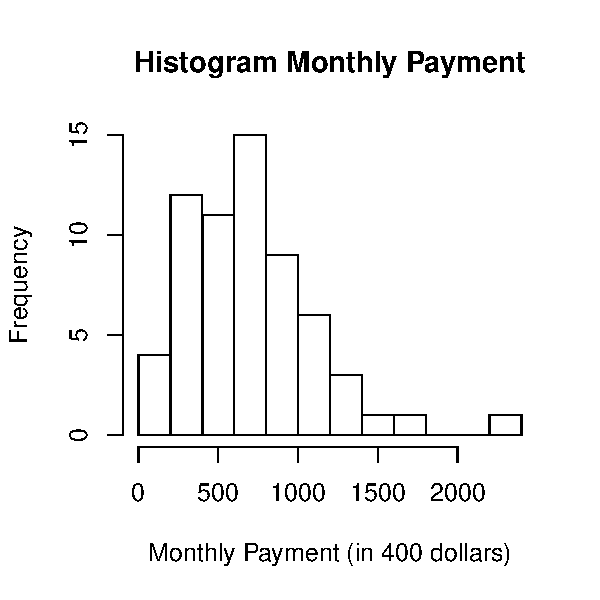
\includegraphics[width=4cm]{figure/LBL2e-1} 


\end{center}
\end{frame}

\begin{frame}[fragile]{iClicker Question 2.4.2}

{\small{
The histogram below shows the BMI (Body Mass Index) of 15  individuals. The right inclusion rule was used in the construction of the  histogram. What class interval(s) occurs least frequently?
}}

\begin{minipage}[ht]{5cm}

{\small{
\begin{enumerate}
\item (25, 30]
\item (30, 35]
\item (20, 25]
\item (25, 30] and (30, 35]
\item Unknown
\end{enumerate}
}}
\end{minipage} \hfill
\begin{minipage}[ht]{6cm}


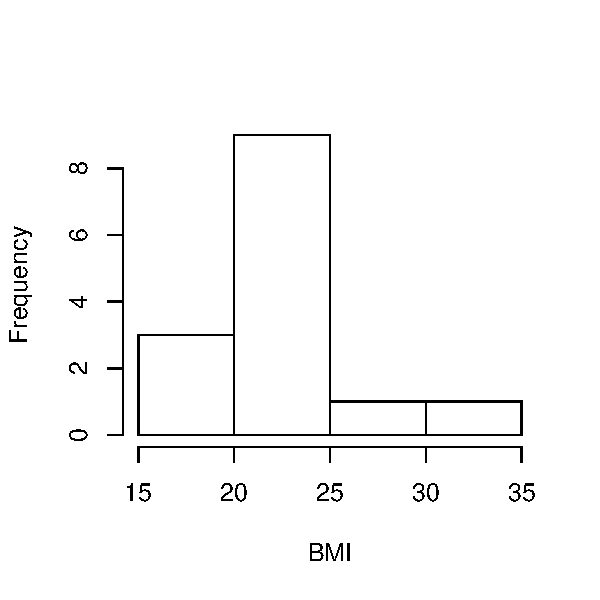
\includegraphics[width=3.5cm]{figure/LBL2f-1} 

\end{minipage}

\end{frame}

\begin{frame}[fragile]{Dotplot}

\begin{itemize}
\item Each observation is represented by a dot, repeated values are  stacked
upwards
\item Below is a comparison dotplot of the monthly payments from the two  types of payment:
\end{itemize}

\begin{figure}[htbp]
   \centering
   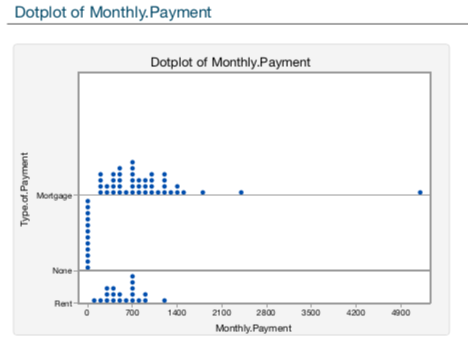
\includegraphics[width=4cm]{chapters/chapter2/ext_figure/dotchart.png} % requires the graphicx package
   %\caption{example caption}
   %\label{fig:example}
\end{figure}
\end{frame}

\begin{frame}[fragile]{iClicker Question 2.4.3}

We summarize numerical data with all of the following EXCEPT:

\begin{enumerate}
\item Bar chart
\item Dotplot
\item Histogram
\item Scatterplot
\item Stem and leaf
\end{enumerate}
\end{frame}


%!Rnw root = ../../Master.Rnw

\section{STAT 1600 Ch 2.4.4 Box and Whisker Plot}

\begin{frame}[fragile]{Statistics and Data Analysis}

STAT 1600 \\
Ch 2.4.4 Box and Whisker Plot

\end{frame}

\begin{frame}[fragile]{Outline}

Summarizing Numerical Data, \#2  

\begin{itemize}
\item Box-and-Whisker Plot  
\item Symmetry and Skewness
\end{itemize}
\end{frame}

\begin{frame}[fragile]{Box -and-whisker plot  (or Boxplot)}

\begin{minipage}[ht]{6cm}

{\small{
This is a graphical picture of the  distribution of quarters of the  data
}}
\end{minipage}
\begin{minipage}[ht]{5cm}


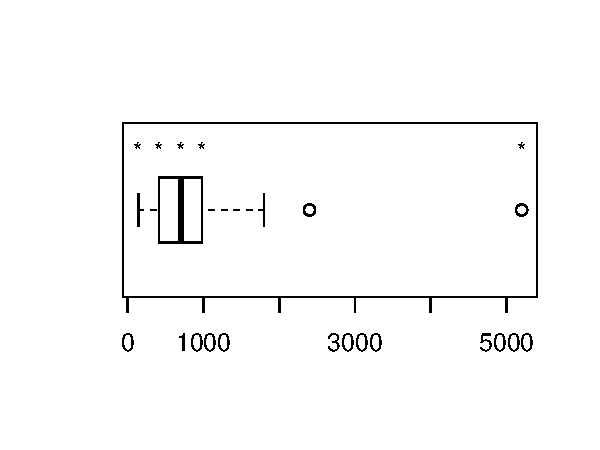
\includegraphics[width=5cm]{figure/LBL2Aa-1} 

\end{minipage}

{\footnotesize{
\begin{itemize}
\item \textbf{This shows the range of each of the four quarters of data:}  
\item MINimum to Q1 (upper boundary of first quarter): 140, 415
\item Median (upper boundary of second quarter, also known as Q2): 700  
\item Q3 is the upper boundary of the third quarter: 975
\item MAXimum is the largest of the ordered observations: 5200
\end{itemize}
}}

\end{frame}

\begin{frame}[fragile]{Five-number Summary}

Payment (Rent/Mortgage, outlier excluded), ACS Data
n = 63;	(n + 1)/4 = 16;	1st quarter of the data 

\vspace{3mm}

140, 190, 200, 200, 220, 230, 250, 280, 290, 340, 340, 350, 370, 380, 380, 400, 420, 440, 450, 490, 500, 500, 500, 510, 530, 550, 560, 650, 670, 670, 700, 700, 700, 700, 710, 720, 740, 740, 750, 760, 770, 800, 850, 880, 900, 900, 910, 970, 990, 1000, 1000, 1100, 1200, 1200, 1200, 1200, 1200, 1300, 1400, 1400, 1500, 1800, 2400, 5200

\vspace{3mm}

The range is from 140 to 415
\end{frame}

\begin{frame}[fragile]{Five-number Summary}

Payment (Rent/Mortgage, outlier excluded), ACS Data
n = 63;	(n + 1)/4 = 16;	2nd quarter of the data 

\vspace{3mm}

140, 190, 200, 200, 220, 230, 250, 280, 290, 340, 340, 350, 370, 380, 380, 400, 420, 440, 450, 490, 500, 500, 500, 510, 530, 550, 560, 650, 670, 670, 700, 700, 700, 700, 710, 720, 740, 740, 750, 760, 770, 800, 850, 880, 900, 900, 910, 970, 990, 1000, 1000, 1100, 1200, 1200, 1200, 1200, 1200, 1300, 1400, 1400, 1500, 1800, 2400, 5200

\vspace{3mm}

The range is from 415 to 700
\end{frame}

\begin{frame}[fragile]{Five-number Summary}

Payment (Rent/Mortgage, outlier excluded), ACS Data
n = 63;	(n + 1)/4 = 16;	3rd quarter of the data 

\vspace{3mm}

140, 190, 200, 200, 220, 230, 250, 280, 290, 340, 340, 350, 370, 380, 380, 400, 420, 440, 450, 490, 500, 500, 500, 510, 530, 550, 560, 650, 670, 670, 700, 700, 700, 700, 710, 720, 740, 740, 750, 760, 770, 800, 850, 880, 900, 900, 910, 970, 990, 1000, 1000, 1100, 1200, 1200, 1200, 1200, 1200, 1300, 1400, 1400, 1500, 1800, 2400, 5200

\vspace{3mm}

The range is from 700 to 975
\end{frame}

\begin{frame}[fragile]{Five-number Summary}

Payment (Rent/Mortgage, outlier excluded), ACS Data
n = 63;	(n + 1)/4 = 16;	4th quarter of the data 

\vspace{3mm}

140, 190, 200, 200, 220, 230, 250, 280, 290, 340, 340, 350, 370, 380, 380, 400, 420, 440, 450, 490, 500, 500, 500, 510, 530, 550, 560, 650, 670, 670, 700, 700, 700, 700, 710, 720, 740, 740, 750, 760, 770, 800, 850, 880, 900, 900, 910, 970, 990, 1000, 1000, 1100, 1200, 1200, 1200, 1200, 1200, 1300, 1400, 1400, 1500, 1800, 2400, 5200

\vspace{3mm}

The range is from 975 to 2400
\end{frame}

\begin{frame}[fragile]{Five-number Summary}

Payment (Rent/Mortgage, outlier excluded), ACS Data
n = 63;	(n + 1)/4 = 16;	In summary,

\begin{itemize} 
\item MIN = smallest observation = 140 
\item Q1  = 1st quartile = 400
\item MED = median (= 2nd quartile) = 700
\item Q3  = 3rd quartile = 970
\item MAX = largest observation = 2400
\item
\item MIN, Q1, MED, Q3, and MAX give five-number summary
\end{itemize}
\end{frame}

\begin{frame}[fragile]{Five-number Summary}

Payment (Rent/Mortgage, outlier excluded), ACS Data
n = 63;	(n + 1)/4 = 16;	In summary,

\begin{itemize} 
\item 50\% of data values $\le$ MED
\item 50\% of data values $\ge$ MED
\item 25\% of data values $\le$ Q1
\item 75\% of data values $\ge$ Q1
\end{itemize}
\end{frame}

\begin{frame}[fragile]{Computing Five-number Summary}

\begin{enumerate}
\item<1-> Sort data into a list of ordered values  
\item<2-> Find MIN and MAX
\item<3-> Determine the sample size (i.e., number of observations) n
\item<4-> Q1 = 0.25(n + 1)th ordered value
\item<5-> MED = 0.5(n + 1)th ordered value
\item<6-> Q3 = 0.75(n + 1)th ordered value
\item<7-> If a non-integer resulted in any computation of the quartiles  (Q1, MED, Q3) above, average the two adjacent ordered  values for the respective quartile
\end{enumerate}
\end{frame}

\begin{frame}[fragile]{Five-number Summary for Monthly Rent}

{\small{
Sorted monthly payments for Type = Rent (n = 20), ACS Data}}

\vspace{3mm}

140, 220, 250, 280, 340, 350, 380, 400, 490, 500, 560, 650, 670, 700, 700, 740, 760, 880, 910, 1200

{\small{
\begin{enumerate}
\item<1-> MIN = 140, MAX = 1200
\item<2-> 0.25(n + 1) = 5.25 and hence Q1 = average of 5th and 6th  ordered values = (340 + 350)/2 = 345
\item<3-> 0.5(n + 1) = 10.5 and hence MED = average of 10th and 11th  ordered values = (500 + 560)/2 = 530
\item<4-> 0.75(n + 1) = 15.75 and hence Q3 = average of 15th and 16th  ordered values = (700 + 740)/2 = 720
\end{enumerate}
}}
\end{frame}

\begin{frame}[fragile]{iClicker Question 2.4.4.1}

 In general, the middle 50\% of data values are bounded by what  statistics?
\begin{enumerate}

\item The first quartile and the median.
\item The first quartile and the third quartile.
\item The median and the third quartile.
\item The median and the maximum.
\item The minimum and the maximum.
\end{enumerate}
\end{frame}

\begin{frame}[fragile]{iClicker Question 2.4.4.2}

Given the 5-Number summary (MIN, Q1, Q2, Q3, and MAX) of any  data set, approximately 75\% of data values are at or above what  statistic?

\begin{enumerate}
\item The median.
\item The first quartile.
\item The third quartile.
\item The maximum.
\item The minimum.
\end{enumerate}
\end{frame}

\begin{frame}[fragile]{Box-and-whisker Plot}


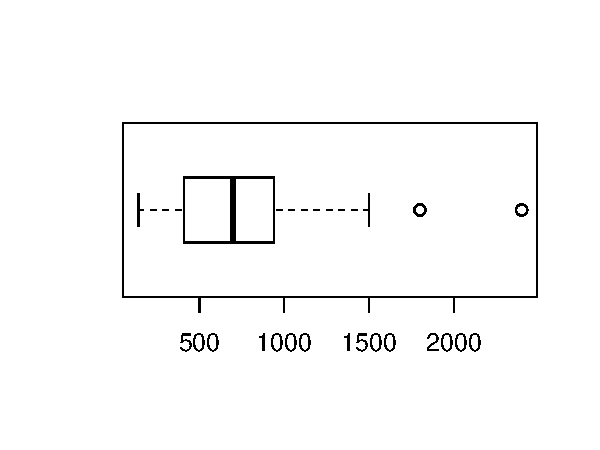
\includegraphics[width=5cm]{figure/LBL2Ac-1} 


\vspace{-8mm}

\begin{itemize}
\item<1-> Draw a horizontal axis covering data range
\item<2-> Draw a box with edges at Q1 and Q3
\item<3-> Draw within the box, a line located at MED
\item<4-> Draw `fences' (lines) at the MIN and MAX
\item<5-> Draw `whiskers' extending from the edges of the box to the MIN and MAX
\end{itemize}
\end{frame}

\begin{frame}[fragile]{Comparison Boxplots}


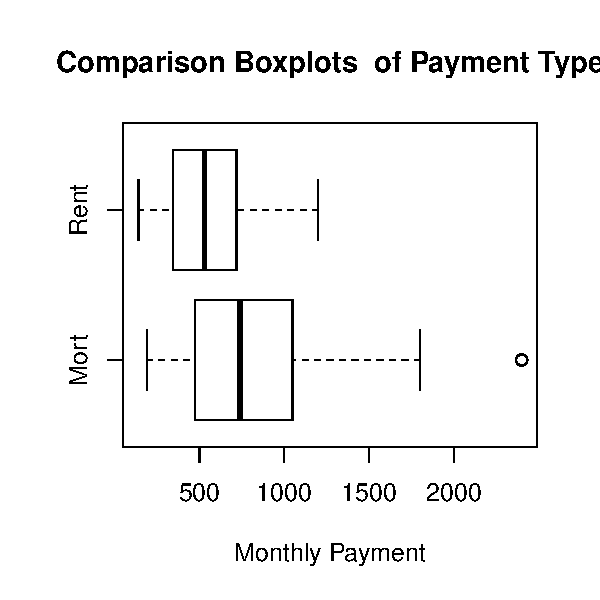
\includegraphics[width=6cm]{figure/LBL2Ad-1} 

\end{frame}

\begin{frame}[fragile]{Symmetry/Skewness}

Left-skewed
{\footnotesize{
\begin{verbatim}


  The decimal point is 1 digit(s) to the right of the |

   4 | 0
   5 | 5
   6 | 2
   7 | 
   8 | 17
   9 | 2445
  10 | 011245569
  11 | 58


\end{verbatim}
}}
\end{frame}

\begin{frame}[fragile]{Symmetry/Skewness}

Symmetric

{\footnotesize{
\begin{verbatim}


  The decimal point is 1 digit(s) to the right of the |

   4 | 7
   5 | 35
   6 | 005
   7 | 00112
   8 | 467899
   9 | 0199
  10 | 14
  11 | 1


\end{verbatim}
}}
\end{frame}

\begin{frame}[fragile]{Symmetry/Skewness}

Right-skewed

{\footnotesize{
\begin{verbatim}


  The decimal point is 1 digit(s) to the right of the |

   4 | 58
   5 | 011245569
   6 | 2445
   7 | 17
   8 | 
   9 | 2
  10 | 5
  11 | 0


\end{verbatim}
}}
\end{frame}

\begin{frame}[fragile]{Symmetry/Skewness, continued}

\begin{itemize}
\item<1-> \textbf{Symmetric:} data shape in two mirror-imaged halves  
\item<2-> \textbf{Right-skewed:} long right tail
\item<3-> \textbf{Left-skewed:} long left tail
\item<4-> \textbf{Symmetry/Skewness} can be detected by inspecting the stem-and-leaf plot (first turn it  counter-clockwise 90 degrees), histogram, dotplot, or boxplot  (median is half way from the edges of the box, whiskers on two sides of equal length)
\end{itemize}
\end{frame}

\begin{frame}[fragile]{iClicker Question 2.4.4.3}

The stem-and-leaf displays of two data sets are given below. Describe  the shape of these two data sets.

\vspace{3mm}

\begin{minipage}[ht]{7.5cm}

\begin{enumerate}
\item 1. symmetric; 2. left skewed
\item 1. right skewed; 2. symmetric
\item 1. symmetric; 2. symmetric
\item 1. left skewed; 2. left skewed
\item 1. symmetric; 2. right skewed
\end{enumerate}
\end{minipage}
\begin{minipage}[ht]{2cm}

{\footnotesize{
\begin{tabular}{@{} r|l @{}} \hline
 & Set 1 \\ \hline
1 & 599 \\
2 & 0113 \\
3 & 669 \\ \hline
\end{tabular}

\begin{tabular}{@{} r|l @{}} \hline
& Set 2 \\ \hline
0 & 1223466 \\
1 & 0015 \\
2 & 9 \\ \hline
\end{tabular}
}}
\end{minipage}
\end{frame}

\begin{frame}[fragile]{iClicker Question 2.4.4.4}

Describe the shape of the box-and-whisker plot (boxplot) below.

\begin{minipage}[ht]{5cm}

{\small{
\begin{enumerate}
\item Symmetric
\item Right skewed
\item Left skewed
\item right and left skewed
\item None of the above
\end{enumerate}
}}
\end{minipage}
\begin{minipage}[ht]{5.5cm}
  

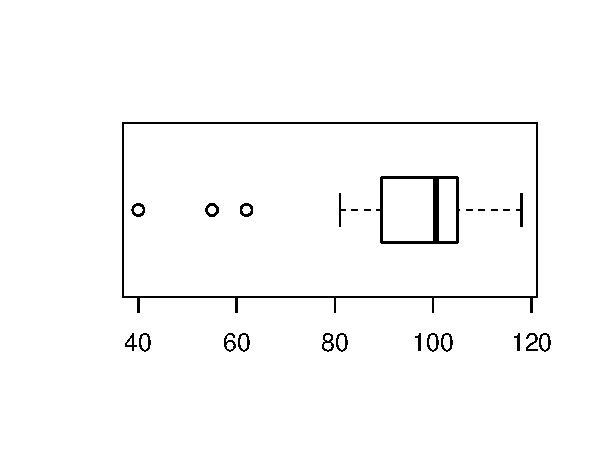
\includegraphics[width=5cm]{figure/LBL2Ae-1} 

\end{minipage}
\end{frame}


%!Rnw root = ../../Master.Rnw

\section{STAT 1600 Ch 2.4.4 Box and Whisker Plot}

\begin{frame}[fragile]{Statistics and Data Analysis}

STAT 1600 \\
Ch. 3 Estimates of Center

\end{frame}

\begin{frame}[fragile]{Outline}

Summarizing Numerical Data, \#3

\begin{itemize}
\item Location and Spread 
\end{itemize}
\end{frame}

\begin{frame}[fragile]{Importance of Location and Spread}


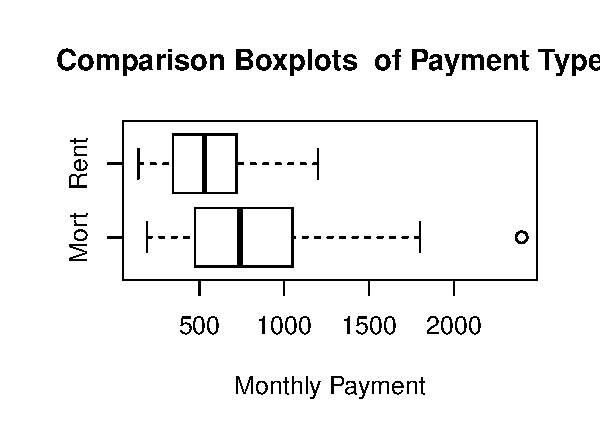
\includegraphics[width=6cm]{figure/LBL3a-1} 


\vspace{-3mm}

{\footnotesize{
\begin{itemize}
\item<1-> The central \textit{location} of Rent appears to be smaller than that of Mortgage
\item<2-> Moreover, the \textit{spread} of Rent appears to be smaller than that of  Mortgage, i.e., Rent payment is less scattered (or less variable)  than that of Mortgage
\item<3-> But how do we quantify such comparisons?  $\Rightarrow$ through \textbf{location} and \textbf{spread} measures
\end{itemize}
}}
\end{frame}

\begin{frame}[fragile]{Outline}

Summarizing Numerical Data, \#3

\begin{itemize}
\item Location and spread
  \begin{itemize}
  \item Location and spread
  \end{itemize}
\item Estimates of Center
  \begin{itemize}
  \item Estimating Average Value
  \item The Sample Means
  \item The Trimmed Mean
  \item The Median of Pairwise Averages
  \end{itemize}
\end{itemize}
\end{frame}

\begin{frame}[fragile]{How do you estimate the average rental}

Based on the following random sample of 2-bedroom apartments in Kalamazoo area

\vspace{3mm}



  650, 400, 740, 880, 500, 350, 280, 380, 250, 220
  
\vspace{3mm}

  How do you measure the (central) location of such rentals?

\end{frame}

\begin{frame}[fragile]{Sample Mean is an Est. of Pop. Mean}

\begin{itemize}
\item<1-> The sample mean (i.e., average of the sample) is denoted by $\bar{X}$
\item<2-> and is the arithmatic average of data values  i.e.,
\item<3->
\begin{equation*}
\bar{X} = \frac{\texttt{sum of data values}}{\texttt{sample size}}
\end{equation*}
\item<4-> (2-bedroom appartment rental example)
\item<5->
\begin{equation*}
\bar{X} = \frac{650 + 400 + \cdots + 220}{10} = 465
\end{equation*}
\end{itemize}

\end{frame}
 
\begin{frame}[fragile]{Sample Mean is an Est. of Pop. Mean}

\begin{itemize}
\item<1-> That is, the average rent for 2-bedroom apartments in  Kalamazoo area is \$ 465 in our sample
\item<2-> This is not to be interpreted as the actual \textit{population average}  (i.e., the actual average rent of all 2-bedroom apartments in  the entire Kalamazoo area)
\item<3-> It is subject to \textit{sampling error}
\item<4-> It likely missed the true population mean \\ (denoted $\mu$), by $| \bar{X} - \mu |$,  the \textit{sampling error}.
\end{itemize}

\end{frame}

\begin{frame}[fragile]{The Sample Median}



{\footnotesize{
\begin{itemize}
\item<1-> an alternative to the sample mean as a measure of location

\item<1-> Recall that the median is the 0.5(n + 1)th ordered data value

\item<1-> Sorted list of Kalamazoo 2-bedroom rental data

\vspace{3mm}

220, 250, 280, 350, 380, 400, 500, 650, 740, 880
\item<2->
\begin{equation*}
0.5(n + 1) = 0.5 \times 11 = 5.5
\end{equation*}

\item<3-> 5.5 is in-between 5 and 6
\item<4-> Hence, MED = average of 5th \& 6th ordered values
\item<5->
\begin{equation*}
\tilde{x} = \frac{ 380 + 400 }{2} = 390
\end{equation*}
\end{itemize}
}}
\end{frame}

\begin{frame}[fragile]{iClicker Question 3.1.1}


The fuel efficiency (MPG) of 5 Japanese made cars are listed below

\begin{center}
27.5, 27.2, 34.1, 29.5, 31.8
\end{center}

What is the median MPG?

\begin{enumerate}
\item 29.5
\item 34.1
\item 30.50
\item 28.5
\item 27.5
\end{enumerate}
\end{frame}

\begin{frame}[fragile]{Sample Mean versus Sample Median}

\begin{itemize}
\item<1-> Sample mean is sensitive to outliers
\item<2-> Sample median is \textit{insensitive} to outliers
\item<3-> In the Kalamazoo apartment rental data, what if the smallest value \$ 220 is replaced by \$100?
\item<4-> The MED remains unchanged (\$ 390) but $\bar{X} = 453$, down by from the original data (\$ 465).
\end{itemize}
\end{frame}

\begin{frame}[fragile]{Sample Mean versus Sample Median}

\begin{itemize}
\item Looking at another example:
\item Let's say we have a dataset of the following:  
\item Data: 5, 10, 17, 20, 25
\item Mean: \textbf{15.4}; Median:17
\item Data: 5, 10, 17, 20, 40
\item Mean: \textbf{18.4};  Median: 17
\end{itemize}

We can see the median has not been affected by the outlier, whereas the  mean has been affected.

\end{frame}

\begin{frame}[fragile]{The Trimmed Mean}


{\small{
\begin{itemize}
\item<1-> The Trimmed Mean is less sensitive to outliers when compared with sample mean  
\item<2-> 10\% trimmed mean = mean of data with lowest 10\% values and  highest 10\% values excluded = mean of middle 80\% values
\item<3-> in Kalamazoo apartment rental data, 10\% of n = 10 is 1 ($n \times 0.1 = 1$)

250, 280, 350, 380, 400, 500, 650, 740
% $500	$500	$525	$555	$635	$650	$670	$675	$750	$800
\item<4-> Hence, 10\% trimmed mean, denoted $\bar{X}_{tr}$, is computed by
\begin{eqnarray*}
\bar{X}_{tr} &=& \frac{250+280+350+380+400+500+650+740}{8} \\
     &=&443.75
\end{eqnarray*}
\end{itemize}
}}
\end{frame}

\begin{frame}[fragile]{The Trimmed Mean -- cont'd}

\begin{itemize}
\item<1-> If $n \times 0.1$ is not an integer, round it up. E.g., if $n = 23$ such that  $n \times 0.1 = 2.3$ then exclude the 3 lowest values and the 3 highest values, thus computing the trimmed mean as the  average of 17 ($= 23 - 3 - 3$) middle values to ensure at least  10\% protection (against outlying values at each end)

\item<2-> The dataset must be ordered.
\end{itemize}

\end{frame}

\begin{frame}[fragile]{The Median of Pairwise Averages}

\begin{itemize}
\item The median of pairwise averages is another  compromise between the mean and the median.
\item We replace observations by pairwise averages of  those observations.
\item Next we take the median of those.
\item Also make sure to pair each observation with  itself!
\item Proceed in the following pattern as laid out on the  next slide.
\end{itemize}
\end{frame}

\begin{frame}[fragile]{The Median of Pairwise Averages}

\begin{table}[ht]
\centering
{\tiny{
\begin{tabular}{@{}cccccccccc @{}} 
$\frac{500+500}{2}$ & $\frac{500+500}{2}$ & $\frac{500+525}{2}$ & $\frac{500+555}{2}$ & $\frac{500+635}{2}$ & $\frac{500+650}{2}$ & $\frac{500+670}{2}$ & $\frac{500+675}{2}$ & $\frac{500+750}{2}$ & $\frac{500+800}{2}$ \\
     & $\frac{500+500}{2}$ & $\frac{500+525}{2}$ & $\frac{500+555}{2}$ & $\frac{500+635}{2}$ & $\frac{500+650}{2}$ & $\frac{500+670}{2}$ & $\frac{500+675}{2}$ & $\frac{500+750}{2}$ & $\frac{500+800}{2}$ \\
     & & $\frac{525+525}{2}$ & $\frac{525+555}{2}$ & $\frac{525+635}{2}$ & $\frac{525+650}{2}$ & $\frac{525+670}{2}$ & $\frac{525+675}{2}$ & $\frac{525+750}{2}$ & $\frac{525+800}{2}$ \\
     & & & $\frac{555+555}{2}$ & $\frac{555+635}{2}$ & $\frac{555+650}{2}$ & $\frac{555+670}{2}$ & $\frac{555+675}{2}$ & $\frac{555+750}{2}$ & $\frac{555+800}{2}$ \\
     & & & & $\frac{635+635}{2}$ & $\frac{635+650}{2}$ & $\frac{635+670}{2}$ & $\frac{635+675}{2}$ & $\frac{635+750}{2}$ & $\frac{635+800}{2}$ \\
     & & & & & $\frac{650+650}{2}$ & $\frac{650+670}{2}$ & $\frac{650+675}{2}$ & $\frac{650+750}{2}$ & $\frac{650+800}{2}$ \\
     & & & & & & $\frac{670+670}{2}$ & $\frac{670+675}{2}$ & $\frac{670+750}{2}$ & $\frac{670+800}{2}$ \\
     & & & & & & & $\frac{675+675}{2}$ & $\frac{675+750}{2}$ & $\frac{675+800}{2}$ \\
     & & & & & & & & $\frac{750+750}{2}$ & $\frac{750+800}{2}$ \\ 
     & & & & & & & & & $\frac{800+800}{2}$ \\
\end{tabular}
}}
\end{table}

{\scriptsize{
\begin{itemize}
\item averaging 1st obs with itself = (500 + 500) / 2 = 500,
\item averaging 1st obs with 2nd obs = (500 + 500) / 2 = 500, and so on ...  
\item averaging 2nd obs with itself = (500 + 500) / 2 = 500, and so on ...  
\item and so on ...
\item median of 55 (= .5(n + 1)/2) pairwise averages = 28th (0.5(55 + 1) = 28)  ordered pairwise average = \$625.0.
\end{itemize}
}}
\end{frame}

\begin{frame}[fragile]{Robustness of Est. of Central Location}

\begin{itemize}
\item Recall that an estimate is robust if it is insensitive to outliers.
\item \textbf{Robust} = resistant to errors
\item The sample mean is NOT robust. That is, it is sensitive to  outliers.
\item The sample median and the median of pairwise averages are  robust.
\item The trimmed means are more robust than the mean but less  robust than the median. Trimmed means with higher trimmed  percentage are more robust.
\end{itemize}
\end{frame}

\begin{frame}[fragile]{Clicker Question 3.1.2}

For estimates of central location, which of the following statements is  true?

\begin{enumerate}
\item Median, mean, and the median of pairwise averages are  robust.
\item Median, 20\% trimmed mean, and mean are robust.
\item Mean and the median are not robust.
\item Median and the median of pairwise averages are robust.
\item All statements above are incorrect.
\end{enumerate}
\end{frame}


%!Rnw root = ../../Master.Rnw

\section{STAT 1600 Ch 3.2 Estimates of Spread}

\begin{frame}[fragile]{Statistics and Data Analysis}

STAT 1600 \\
Ch 3.2 Estimates of Spread 

\end{frame}

\begin{frame}[fragile]{Outline}

Estimates of Spread  

\begin{itemize}
\item Estimates of Spread
\item The Sample Standard Deviation
\item Effect of Multiplication/Addition by a Constant 
\end{itemize}
\end{frame}

\begin{frame}[fragile]{Estimates of Spread }

(or Uncertainty, Variation)

\begin{itemize}
\item<1-> An estimate of spread is a measure of uncertainty, or  variation, or `give or take'
\item<2-> When two or more comparable data sets (comparable means data sets are of same type/same unit of numerical  measurements) are compared, the one with the smallest spread has the least uncertainty around the estimate of center (i.e., least  scattered)
\item<3-> Estimates of spread are non-negative
\end{itemize}
\end{frame}

\begin{frame}[fragile]{Estimates of Spread, Cont'd}

 i.e., 
 
\begin{itemize} 
\item<1-> The standard deviation (SD) is typically used as a `give or  take' number in describing the spread of a dataset 
\item<2->
\begin{equation*}
\texttt{Sample SD} = s = \sqrt{ \frac{ \sum (X - \bar{X})^2}{n - 1}} = \sqrt{ \frac{SS}{n -1}}
\end{equation*}
\end{itemize}
\end{frame}



\begin{frame}[fragile]{The Sample Standard Deviation (SD)}

\begin{minipage}[ht]{5cm}

{\footnotesize{
% latex table generated in R 3.5.1 by xtable 1.8-2 package
% Sun Jul 22 19:18:43 2018
\begin{table}[ht]
\centering
\begin{tabular}{rrrr}
  \hline
 & Rent & Diff & Diff Sqd \\ 
  \hline
1 & 650 & 185 & 34225 \\ 
  2 & 400 & -65 & 4225 \\ 
  3 & 740 & 275 & 75625 \\ 
  4 & 880 & 415 & 172225 \\ 
  5 & 500 & 35 & 1225 \\ 
  6 & 350 & -115 & 13225 \\ 
  7 & 280 & -185 & 34225 \\ 
  8 & 380 & -85 & 7225 \\ 
  9 & 250 & -215 & 46225 \\ 
  10 & 220 & -245 & 60025 \\ 
   \hline
\end{tabular}
\end{table}

}}

\end{minipage}
\begin{minipage}[ht]{6cm}

{\footnotesize{
\begin{itemize}
\item<1-> Step 1. Compute $\bar{x} = 465$
\item<2-> Step 2. Calculate Diff, i.e., how much an obs. `missed by' the average, (i.e., deviation).
\item<3-> Step 3. Square the `missed by' differences.
\item<4-> Step 4. Add all the squared `missed by' differences, i.e., SS
\item<5-> Step 5. Take the square-root of $\frac{SS}{n - 1}$ to get SD

\begin{equation*}
SD = \sqrt{ \frac{\ensuremath{4.4845\times 10^{5}}}{ 10 - 1 }} = 223.2
\end{equation*}

\end{itemize}
}}
\end{minipage}

\end{frame}

\begin{frame}[fragile]{Interpretation of SD}



{\small{
\begin{table}
\caption{Bowling Example}
\begin{tabular}{@{} lc | c c @{}} \hline
Games & Scores & Mean & SD \\ \hline
First games & 163, 231, 224, 238, 279, 239, 226 & 228.6 & 34.34 \\
Last games  & 246, 244, 247, 248, 237, 258, 246 & 246.6 & 6.21 \\ \hline
\end{tabular}
\end{table}

Scores of Walter Ray Williams Jr. in 2008 bowling  tournament, Indiana

}}
\end{frame}

\begin{frame}[fragile]{Interpretation of SD}

{\footnotesize{
Scores of Walter Ray Williams Jr. in 2008 bowling  tournament, Indiana 


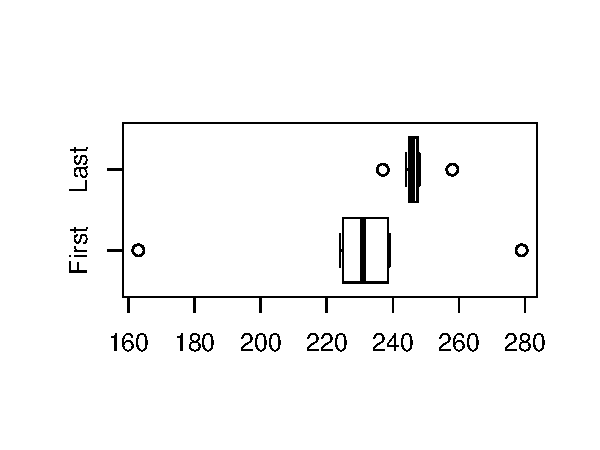
\includegraphics[width=6cm]{figure/LBLAc-1} 


\begin{itemize}
\item Bigger swings (larger SD) in earlier games and scored typically lower  (smaller Mean)
\item He played consistently (smaller SD) in later games, and typically with  better scores (larger Mean)
\end{itemize}
}}
\end{frame}

\begin{frame}[fragile]{Sample Standard Deviation is Not Robust}

As an estimate of the spread of a data set, the sample standard  deviation \textbf{is sensitive to outliers}.

\end{frame}

\begin{frame}[fragile]{iClicker Question 3.2.1}

The fuel efficiency (MPG) of 5 Japanese made cars are listed below

27.5,	27.2,	34.1,	29.5,	31.8

Ignoring any rounding error, what is the sum of all the deviations (MPG  for Japanese made cars) from the mean MPG for Japanese made  cars?

\begin{enumerate}
\item 9.38
\item 4.19
\item 0.00
\item -4.19
\item 30.58
\end{enumerate}
\end{frame}

\begin{frame}[fragile]{iClicker Question 3.2.2}

Recall that an estimate is robust if it is insensitive to outliers. Which of  the following statements is true.

\begin{enumerate}
\item The sample mean and the standard deviation are robust.
\item The sample mean is robust but the standard deviation is  not.
\item The sample mean is not robust but the standard deviation  is.
\item The sample mean and the standard deviation are not  robust.
\item None of the previous statements is true.
\end{enumerate}
\end{frame}

\begin{frame}[fragile]{Effect of Multiplication/Addition by a Constant}



\begin{center}
apartment rental example
\end{center}

\begin{itemize}
\item<1-> Recall that the mean and SD are \$ $465 \pm 223.2$ \\ ($\pm$ means `give or take')
\item<2-> Get a roommate and pay half the rent: \$ $232.5 \pm 111.6$ %$323  ± $52
\item<3-> No roommate but has contribution of \$100 per month from parents: $232.5 \pm 223.2$    % $526 ± $104
\end{itemize}
\end{frame}

\begin{frame}[fragile]{General Rules}

\begin{itemize}
\item<1-> when a constant is \textbf{added to/subtracted from} each data  value, the same thing happens to the average, but the SD  remains unchanged,
\item<2-> when each data value is \textbf{multiplied or divided} by a positive  constant, the same thing happens to both the average and  the SD.
\end{itemize}
\end{frame}

\begin{frame}[fragile]{General Rules}

\begin{minipage}[ht]{5cm}

{\small{
Eg. data: 1, 2, 3

\begin{tabular}{@{} ccc @{}} \hline
X & Diff & Sqd \\ \hline
1 & -1 & 1 \\
2 & 0 & 0 \\
3 & 1 & 1 \\ \hline
$\bar{x}=2$ & 0 & $SS=2$ \\ \hline
\end{tabular}

\begin{equation*}
SD = \sqrt{ \frac{2}{(3-1)}} = 1
\end{equation*}
}}
\end{minipage}
\begin{minipage}[ht]{5cm}
{\small{
Eg. data: 3, 4, 5 (added 2)

\begin{tabular}{@{} ccc @{}} \hline
X & Diff & Sqd \\ \hline
3 & -1 & 1 \\
4 & 0 & 0 \\
5 & 1 & 1 \\ \hline
$\bar{x}=4$ & 0 & $SS=2$ \\ \hline
\end{tabular}

\begin{equation*}
SD = \sqrt{ \frac{2}{(3-1)}} = 1
\end{equation*}
}}
\end{minipage}

Notice here the mean increased from 2 to 4, yet the SD did not change.

\end{frame}

\begin{frame}[fragile]{General Rules}

\begin{minipage}[ht]{5cm}

{\small{
Eg. data: 1, 2, 3

\begin{tabular}{@{} ccc @{}} \hline
X & Diff & Sqd \\ \hline
1 & -1 & 1 \\
2 & 0 & 0 \\
3 & 1 & 1 \\ \hline
$\bar{x}=2$ & 0 & $SS=2$ \\ \hline
\end{tabular}

\begin{equation*}
SD = \sqrt{ \frac{2}{(3-1)}} = 1
\end{equation*}
}}
\end{minipage}
\begin{minipage}[ht]{5cm}
{\small{
Eg. data: 2, 4, 6 (times 2)

\begin{tabular}{@{} ccc @{}} \hline
X & Diff & Sqd \\ \hline
2 & -2 & 4 \\
4 & 0 & 0 \\
6 & 2 & 4 \\ \hline
$\bar{x}=4$ & 0 & $SS=8$ \\ \hline
\end{tabular}

\begin{equation*}
SD = \sqrt{ \frac{4}{(3-1)}} = 2
\end{equation*}
}}
\end{minipage}

In this second example, multiplying by 2 the mean doubled AND the SD doubled.

\end{frame}

\begin{frame}[fragile]{iClicker Question 3.2.3}

Compute the mean given the following data:

8, 12, 15, 22, 28

\begin{enumerate}
\item 5
\item 10
\item 15
\item 17
\item 20
\end{enumerate}
\end{frame}


%!Rnw root = ../../Master.Rnw

\section{STAT1600 Ch 4 Threats to Valid Comparisons}

\begin{frame}[fragile]{Statistics and Data Analysis}

STAT1600 \\ Ch 4 Threats to Valid Comparisons

\end{frame}

\begin{frame}[fragile]{Outline}

Threats to Valid Comparisons  

\begin{itemize}
\item Hidden Confounder
\end{itemize}
\end{frame}

\begin{frame}[fragile]{Hidden Confounder}

Lower Extremity Fractures Example

In the study of `Lower extremity fractures in motor vehicle collisions:  Influence of direction of impact and seatbelt use,' one of the  conclusions is of interest: there was a higher incidence of lower  extremity fracture among women.

\end{frame}

\begin{frame}[fragile]{Lower Extremity Fractures}

Wrong assumptions may lead to wrong conclusions

by falsely assuming that gender \textbf{causes} higher/lower leg fractures, one  may reach these \textbf{false conclusions} about the study outcome `women  have higher rates of leg fractures'

\begin{itemize}
\item because they drive faster?  
\item apply brakes more slowly?  
\item have weaker bones?
\end{itemize}
\end{frame}

\begin{frame}[fragile]{Lower Extremity Fractures}

{\small{
A follow-up study titled `the role of driver gender and height'

turns out that \textbf{height} was the culprit.\\
Because \textbf{height} and \textbf{gender} have a strong link, a false conclusion  can result from a false assumption.\\
The pathway graph below describes the true relationship:

\vspace{3mm}

\begin{tabular}{@{} lllll @{}} 
\texttt{Confounder} & \texttt{Height} & $\Rightarrow$ & \texttt{Leg Fracture} & \texttt{Outcome} \\
\texttt{(actual cause)} & $\updownarrow$ &  & \\
\texttt{Prob cause} &\texttt{Gender} & &
\end{tabular}

\vspace{3mm}

$\updownarrow$  Means `association' or `probable cause' \\
$\Rightarrow$  Means `cause-and-effect'
}}
\end{frame}

\begin{frame}[fragile]{Lower Extremity Fractures}

\begin{tabular}{@{} lllll @{}} 
 & \texttt{Height} & $\Rightarrow$ & \texttt{Leg Fracture}  \\
\texttt{pathway graph :} & $\updownarrow$ &  & \\
 &\texttt{Gender} & &
\end{tabular}

\begin{itemize}
\item outcome variable: leg fracture.
\item probable cause: gender.
\item confounder or confounding variable: the hidden variable height.
\end{itemize}
\end{frame}

\begin{frame}[fragile]{Confounding Variable or Confounder}

A \textbf{confounder} is a third variable that is associated with both the probable cause and  the \textbf{outcome}.

\begin{itemize}
\item \textit{Overlooking} its existence can lead us to drawing a \textit{wrong  conclusion} about the cause-and-effect relationship.
\item Hidden confounders are one of the biggest sources of (often  unknowingly) \textit{invalid comparisons}. One could end up comparing  apples to oranges! (Note: women as a group are shorter than men!)
\end{itemize}
\end{frame}

\begin{frame}[fragile]{Lower Extremity Fractures, cont'd}

Potential confounders other than height includes 

\begin{itemize}
\item weight,  
\item none/light/heavy smoker, 
\item alcohol consumption, 
\item short/long hair,  
\item wearing higher heels or not, 
\item ..., etc.
\end{itemize}
\end{frame}

\begin{frame}[fragile]{iClicker Question 4.1}

According to ``Cumulative Use of Strong Anticholinergics and Incident  Dementia'' (JAMA, March 2015), from 10 years of tracking older adults  and their use of anticholinergic drugs (meant to reduce symptoms of  allergies, inability to sleep, anxiety, depression and bladder over-activity), the risk of Alzheimer's was 63 percent higher. Which of  the following is the \textbf{outcome variable} (response)?

\begin{enumerate}
\item use of anticholinergic drugs
\item risk of Alzheimer's
\item hidden variables such as high blood pressure
\item none of the previous
\end{enumerate}
\end{frame}

\begin{frame}[fragile]{iClicker Question 4.2}

According to ``Cumulative Use of Strong Anticholinergics and Incident  Dementia'' (JAMA, March 2015), from 10 years of tracking older adults  and their use of anticholinergic drugs (meant to reduce symptoms of  allergies, inability to sleep, anxiety, depression and bladder over-activity), the risk of Alzheimer's was 63 percent higher. Which of  the following is the \textbf{probable cause}?

\begin{enumerate}
\item use of anticholinergic drugs
\item risk of Alzheimer's
\item hidden variables such as high blood pressure
\item none of the previous
\end{enumerate}
\end{frame}

\begin{frame}[fragile]{Outline}

Threats to Valid Comparisons  

\begin{itemize}
\item[1] Hidden Confounder
\item[2] In the Headlines
\end{itemize}
\end{frame}

\begin{frame}[fragile]{Examples In the Headlines}

\begin{itemize}
\item<1-> Smoking `causes' lung cancer. True? Having lung cancer or not is  the outcome variable, smoking is probable cause, potential  confounders abound. (see textbook)
\item<2-> not true for a single study or a few studies.
\end{itemize}
\end{frame}

\begin{frame}[fragile]{Examples In the Headlines}

\begin{itemize}
\item<1-> ``Older Viagra Users More Likely to Get STDs'' -- the Chicago Sun  Times and the like. See critiques by Rebecca Goldin and Jing  Peng in August 2010 from  \texttt{http://www.stats.org} titled `If you  take Viagra, will you get an STD?' Pathway graph for this is `person type' (i.e. lifestyle) is a confounder which is the cause (or surrogate of causes)
\item<2-> `taking ED drugs or not' is only a probable cause
\end{itemize}
\end{frame}


%!Rnw root = ../../Master.Rnw

\section{STAT1600 Ch 5 Study Designs}

\begin{frame}[fragile]{Statistics and Data Analysis}

STAT1600 \\ Ch 5 Study Designs

\end{frame}

\begin{frame}[fragile]{Outline}

Study Designs  

\begin{itemize}
\item Randomized Trials
\item Double-blind Randomized Controlled Trials  
\item Observational Studies
\item iClicker Questions
\end{itemize}
\end{frame}

\begin{frame}[fragile]{Diet Comparison Example}

The diet comparison example ``Comparison of the Atkins, Zone,  Ornish, and LEARN Diets for Change in Weight and Related Risk  Factors Among Overweight Premenopausal Women The A TO Z  Weight Loss Study: A Randomized Trial'' by C.D. Gardner, et al.  (JAMA, Vol. 297, pp. 969–977, March 2007) is a good example of  \textbf{randomized trials}.

An important characteristic of the experiment is that the comparison  groups are similar to each other in all aspects, \textbf{except for the  treatment} (see Table 5.1 on page 79). Hence such experiment offers  fair comparison of the treatment among the four diet groups.
\end{frame}

\begin{frame}[fragile]{Randomization and Randomized Trials}

\begin{itemize}
\item<1-> In a randomized trial, subjects entering the trial in a randomized  fashion (using virtual roll of a die) into one of several treatment groups.  This process is called:

\item<2-> Randomization

\item<3-> the best way to safeguard against potential confounders so that the  comparison groups are similar in all factors except for the treatment  itself.
\end{itemize}
\end{frame}

\begin{frame}[fragile]{Randomized Controlled Experiment (or Trial)}

is a randomized experiment in which one of the comparison groups is  a control group or placebo group.
\end{frame}

\begin{frame}[fragile]{Double-blind Randomized Controlled Trial}

is a randomized controlled trial in which neither doctor (the  experimenter) nor patient (experimental subject) knows what treatment  the patient receives.

\begin{itemize}
\item<1-> done by giving the patient a pill that looks/smells... like the  treatment pill, but is actually an inert pill or placebo.
\item<2-> Blinding achieves additional protection against bias.
\item<3-> All groups have the same frame of mind (as opposed to knowing  you are not really getting the new drug)
\item<4-> The experimenter has the same frame of mind evaluating patients  from each group.
\end{itemize}
\end{frame}

\begin{frame}[fragile]{Leg Fracture Example}

In many cases, randomization cannot be achieved in that the  treatments being compared cannot be assigned, e.g., the study  involving women and leg fractures. When a new subject enters the  study (by having a car accident), we observe what gender they belong  to, instead of randomly assigning it. This is an example of  \textit{observational studies}.
\end{frame}

\begin{frame}[fragile]{Typical Reasons for Observational Studies}

{\footnotesize{
\begin{itemize}
\item<1-> Assigning treatment is impossible \\
E.g. to compare fracture rates between men and women, we  cannot randomize subjects into the comparison groups
\item<2-> Assigning treatment is unethical \\
E.g. to compare cancer rates of smokers and nonsmokers, we do  not want to \textit{randomize} subjects into smoker-nonsmoker comparison groups
\item<3-> Assigning treatment is impractical \\
E.g. the outcome is a rare event like cancer or stroke, and a  randomized trial would need too many subjects and too much  time.
\item<4-> In cases like these, a case-control study is generally the way to go.
\end{itemize}
}}
\end{frame}

\begin{frame}[fragile]{Case-control Study}

{\footnotesize{
\textit{starts with the outcome} and then works backward to the type of treatment. For instance in the diet comparison trial, a case-control study would look for people in the population who lost weight, and then ask them what diet they used.

\vspace{3mm}

Case-control studies, compared to randomized controlled experiments,

\begin{itemize}
\item<1-> are frequently used because they are cheaper and easier to conduct;  
\item<2-> are less time-consuming to conduct;
\item<3-> are able to conclude a link or `association,' but are not able to prove  `causation;'
\item<4-> provide initial evidence that can generate resources for more rigorous  studies like double-blind randomized controlled trials.
\end{itemize}
}}
\end{frame}

\begin{frame}[fragile]{Successful Story of a Case-control Study}

The first study formally linking lung cancer to smoking was a 1950  case-control study ``Smoking and Carcinoma of the Lung'' by Richard  Doll and A. Bradford Hill (British Medical Journal, 1950 September 30;  2(4682): page 739–748). This study led to numerous studies, and  consequently, it is now accepted by the scientific community that  smoking causes lung cancer.

\end{frame}

\begin{frame}[fragile]{Case-crossover Study}

allows subjects in the treatment group `cross over' to the control group  an vice versa. That is, each subject can be their own control.

\vspace{3mm}

A successful example: a 1997 study linking cell phone use to car  accidents: ``Association between cellular-telephone calls and motor  vehicle collisions'' by D.A. Redelmeier and R.J. Tibshirani (The New  England Journal of Medicine, 1997 Feb 13; vol 336, pp. 453–458).
\end{frame}

\begin{frame}[fragile]{iClicker Question 5.1}

According to ``Cumulative Use of Strong Anticholinergics and Incident  Dementia'' (JAMA, March 2015), from 10 years of tracking older adults  and their use of anticholinergic drugs (meant to reduce symptoms of  allergies, inability to sleep, anxiety, depression and bladder over-activity), the risk of Alzheimer's was 63 percent higher. What type  of study is this?

\begin{enumerate}
  \item randomized controlled experiment
  \item case-control study
  \item none of the previous
\end{enumerate}
\end{frame}

\begin{frame}[fragile]{iClicker Question 5.2}

Which of the following is \textit{false} about a case-control study when it is  compared to a randomized controlled trial?

\begin{enumerate}
  \item case-control study is less time-consuming to conduct
  \item case-control study is cheaper to conduct
  \item case-control study can be used to determine causation
  \item case-control study is easier to conduct
\end{enumerate}
\end{frame}

\begin{frame}[fragile]{iClicker Question 5.3}

A clinical trial was conducted in which 120 patients with similar clinical  features were randomly divided into a control group and a treatment  group, each consisting of 60 patients. What type of study this is?

\begin{enumerate}
  \item randomized controlled trial
  \item case-control study
  \item none of the previous
\end{enumerate}
\end{frame}

\begin{frame}[fragile]{iClicker Question 5.4}

{\footnotesize{
Western Michigan University offers a 1 credit course for freshmen, UNIV 1010, which teaches about university resources and study habits for success in college. It is an elective course and about half of the freshmen take it. WMU has studied the results by comparing the retention and GPAs of students who took this class against those who did not take this class. It was found that retention and GPAs were generally higher for those who took UNIV 1010. This evidence was put forth as proof that the course was successful and that it should be continued. \\
What potential source(s) of bias have not been accounted for by WMU?

\begin{enumerate}
  \item GPAs before college.
  \item Lack of randomization in subject selection for UNIV 1010
  \item Chosen majors of the students
  \item All the above
\end{enumerate}
}}
\end{frame}


%!Rnw root = ../../Master.Rnw

\section{STAT 1600 Ch. 6 The Normal Distribution}

\begin{frame}[fragile]{Statistics and Data Analysis}

STAT 1600 \\ Ch. 6 The Normal Distribution

\end{frame}

\begin{frame}[fragile]{Outline}

The Normal Distribution

\begin{itemize}
\item Normal Distribution and Z Score
\item Using the Normal or Z Curve
\end{itemize}
\end{frame}

\begin{frame}[fragile]{Normal Distribution}

\begin{minipage}[ht]{5cm}

{\footnotesize{
\begin{itemize}
\item Normal distribution is denoted by N(mean,SD).
\item Standard normal has mean=0 and SD=1 and is denoted  by N(0, 1)z s
\item The mean gives the location of the line of symmetry and the standard deviation refers to the spread. 
\item \textbf{The area  under the curve always equals 1.}
\end{itemize}
}}
\end{minipage}
\begin{minipage}[ht]{5cm}


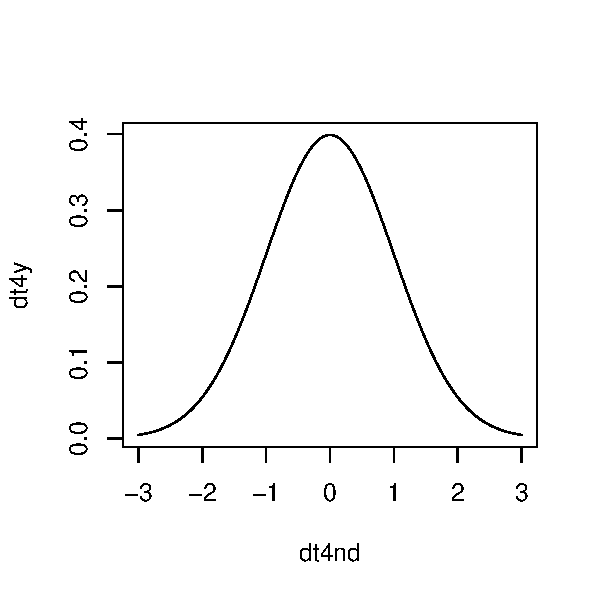
\includegraphics[width=5cm]{figure/LBL6a-1} 


\end{minipage}
\end{frame}

\begin{frame}[fragile]{Normal Distribution}

The normal or bell-shaped curve is helpful in calculating  probabilities

\begin{itemize}
\item 68\% of the data falls within -1 and +1 standard  deviations of the mean
\item 95\% falls between -2 and +2 standard deviations
\item 99.7\% falls between -3 and +3 standard deviations
\end{itemize}
\end{frame}

\begin{frame}[fragile]{Normal Distribution}

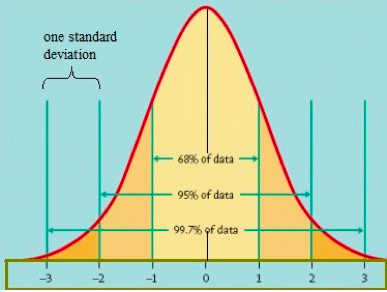
\includegraphics[width=8cm]{chapters/chapter6/ext_figure/norm1.png}

\end{frame}

\begin{frame}[fragile]{Normal Distribution}

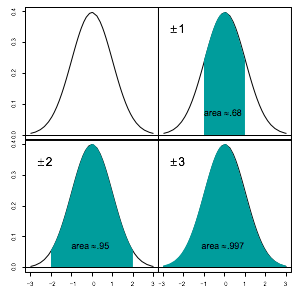
\includegraphics[width=7.5cm]{chapters/chapter6/ext_figure/norm2.png}

\end{frame}

\begin{frame}[fragile]{Normal Distribution}

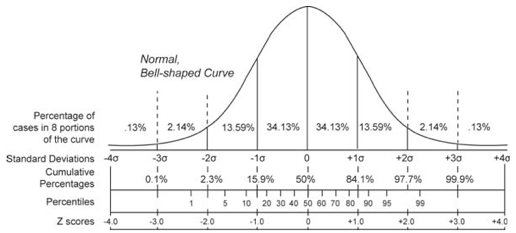
\includegraphics[width=10cm]{chapters/chapter6/ext_figure/norm3.png}

\end{frame}

\begin{frame}[fragile]{Z-score}

{\small{
\begin{itemize}
\item<1-> To calculate area under curve of general N(mean, SD), calculate z  score (i.e., number of SD's above average/below the average).  For example, the area to  the left of X in this normal:

\item<2-> 
\begin{equation*}
  \texttt{calculate z-score of x} = z = \frac{x - \mu}{\sigma} 
\end{equation*}

\item<3-> To find the probability of a random variable, X, occurring in a  normal distribution, we make use of the normal distribution or  normal curve. Once we obtain a z-score using the formula  above we can find the probability of a data value occuring at or  below that value.
\end{itemize}
}}
\end{frame}

\begin{frame}[fragile]{Z-score}

\begin{itemize}
\item To calculate area under curve of general N(mean, SD), calculate z  score (i.e., number of SD's above average/below the average).  For example, the area to  the left of X in this normal:

\item
\begin{equation*}
  \texttt{calculate z-score of x} = z = \frac{x - \mu}{\sigma} 
\end{equation*}

\item then area to the left of x in N(mean, SD) = area to the left of z in N(0,1)
\end{itemize}
\end{frame}

\begin{frame}[fragile]{Z-score}

{\small{
Let X =adult male height. Then X is N (70'', 4''). This is stating that  for this population the mean height in males is 70 inches and the  standard deviation is 4 inches. What is the probability that a male  is less than 6' tall (or 72 inches)?:
}}

\begin{minipage}[ht]{5cm}

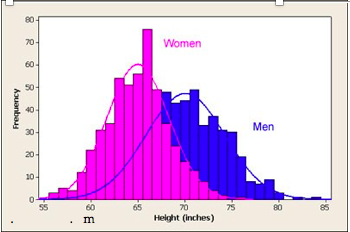
\includegraphics[width=5cm]{chapters/chapter6/ext_figure/norm4.png}


\end{minipage}
\begin{minipage}[ht]{5cm}

\begin{eqnarray*}
z &=& \frac{x - \mu}{\sigma} \\
  &=& \frac{x - 70}{4} \\
  &=& \frac{72 - 70}{4} \\
  &=& 0.5
\end{eqnarray*}
\end{minipage}
\end{frame}

\begin{frame}[fragile]{Z-Score}

{\footnotesize{
Let X = adult male height. Then X is N (70'', 4''). This is stating that  for this population the average height in males is 70 inches and the standard deviation is 4 inches.  What is the probability that a male is less than 6' tall (or 72 inches)?:  }}
 
\begin{minipage}[ht]{5cm}

{\footnotesize{
\begin{eqnarray*}
z &=& \frac{X - \mu}{\sigma} \\
  &=& \frac{X - 70}{4} \\
  &=& \frac{72 - 70}{4} \\
  &=& 0.5 
\end{eqnarray*}
}}
\end{minipage}
\begin{minipage}[ht]{4cm}


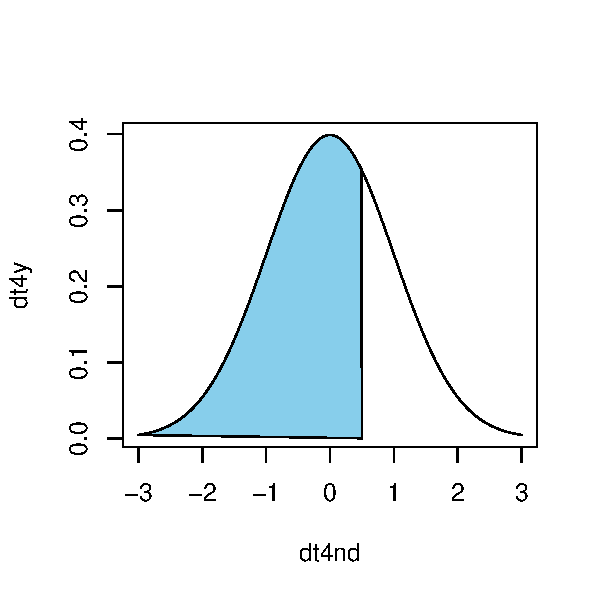
\includegraphics[width=4cm]{figure/LBL6b-1} 

\end{minipage}

{\footnotesize{
A Z value of 0.5 corresponds to the area of 0.6915 (AUC).  This means the probability, $P(X \le 72$ inches), is 69.15\%
}}
\end{frame}


%!Rnw root = ../../Master.Rnw

\section{Stat1600 Ch 7 The Binomial Distribution}

\begin{frame}[fragile]{Statistics and Data Analysis}

STAT 1600 \\ Ch 7 The Binomial Distribution

\end{frame}

\begin{frame}[fragile]{Outline}

The Binomial Distribution  

\begin{itemize}
\item Binomial Random Variables
\end{itemize}
\end{frame}

\begin{frame}[fragile]{Binomial Process and Binomial RV}


A sequence of (fixed) n observations is called a \textbf{binomial process} if

\begin{itemize}
\item<2-> each observation results in exactly one of two possible outcomes  (conveniently called \textit{success} and \textit{failure})
\item<2-> P (success) = p, and P (failure) = q = 1 - p for all observations  
\item<2-> observations are independent
\item<3-> X = total number of successes among the n observations is a  \textbf{binomial random variable} with parameters n and p and is denoted  $X \sim binomial(n, p)$
\end{itemize}

\end{frame}

\begin{frame}[fragile]{Binomial Process and Binomial RV}


Example: What is the probability of rolling exactly two ones in 10  rolls of a die? (n, our sample size = 10)

There are several things you need to know:  

\begin{enumerate}
\item First Define Success: "Rolling a 1 on a single die"

\item Define the probability of success: (p): $p = \frac{1}{6} = 0.167$ 

\item Find the probability of failure: $(1 - p) = q = \frac{5}{6} = 0.833$ 

\item Define the X (or j) that we are investigating.  This is the number of successes out of the trials(or sample size, n):  Here it is two rolls out of 10 so $X = j = 2$
\end{enumerate}

\end{frame}

\begin{frame}[fragile]{Binomial Process and Binomial RV}

\begin{itemize}
\item<1-> Example: \textbf{What is the probability of rolling exactly two ones in 10  rolls of a die?}  Anytime a `1' appears it is a success.  Anytime any other number  (2, 3, 4, 5, 6) appears it is a failure.
\item<2-> We need to use the binomial probability distribution  function in order to solve for this:
\item<3->
\begin{equation*}
P[ X = j] = \frac{n!}{j! (n - j)!} p^j (1 - p)^{n - j}, 
\end{equation*}

\texttt{where j = 0, 1, 2, $\cdots$, n}
\end{itemize}
\end{frame}

\begin{frame}[fragile]{Binomial Process and Binomial RV}

In our example: \\
X = j = 2 and  n = 10 \\
p = (probability of success) = 1/6 = 0.167 \\
q = (probability of failure) = 1 - p = 1 - 0.167 = 0.833 \\
(Since q is the probability of failure in our example you can see it is also 5/6 as there are five other numbers the die could fall on.)
\end{frame}

\begin{frame}[fragile]{Using Formula to Compute Binomial Probability}

$X \sim binomial(n, p)$

\begin{eqnarray*}
P[X = 2] &=& \frac{10!}{2! (10 - 2)!} (.167)^2 (.833)^{10-2} \\
   &=& \frac{ 10 \times 9 \times 8!}{ (2 \times 1) (8!)} (.167)^2 (.833)^{8} \\
   &=& (45)(.167)^2 (.833)^{8} \\
   &=& 0.291 \texttt{ or } 29.1\%
\end{eqnarray*}

\end{frame}

\begin{frame}[fragile]{Examples of Binomial RV}

\begin{itemize}
\item A 5-question multiple-choice quiz has 5 choices on each question.
X = number of correct answers (success = correct) in the quiz by
guessing all.  Then $X \sim binomial( n = 5, p = 0.20)$.

\item Past experience: 40\% phone respondents agree to be interviewed  (success = a respondent agrees to be interviewed) for market  research survey. Of 50 reached by Reliable Research, X respondents agree to be interviewed. Then
$X \sim binomial(n = 50, p = 0.40)$.

\end{itemize}
\end{frame}

\begin{frame}[fragile]{Examples of Binomial RV}

\begin{itemize}

\item Suppose historical data shows that 20\% of buyers at Best Buy who purchase smart fitness and GPS watches also purchase the Geek Squad’s extended protection plan (success = a buyer purchases extended protection plan). X extended protection plans were sold along with the 300 smart watches sold last quarter. Then $X \sim binomial(n = 300, p = 0.20)$.

\end{itemize}
\end{frame}

\begin{frame}[fragile]{iClicker Question 7.1}

The probability that a defective item is observed at a production line  is 0.02. A quality engineer, working at the production line, inspects  an item. What is the chance that the item is found to be non-defective?

\begin{enumerate}
\item 0.02
\item 1
\item 0.98
\item -0.02
\item none of the previous
\end{enumerate}
\end{frame}

\begin{frame}[fragile]{iClicker Question 7.2}

Over a long period of time in a large multinational corporation, 10\% of all sales trainees are rated as outstanding, 75\% are rated as excellent/good, 10\% percent are rated as satisfactory, and 5\% are considered unsatisfactory. What is the probability that a sales trainee is rated as not outstanding?

\begin{enumerate}
\item 0.05
\item 0.10
\item 0.25
\item 0.90
\item 0.95
\end{enumerate}
\end{frame}

\begin{frame}[fragile]{Outline}

The Binomial Distribution  

\begin{itemize}
\item Binomial Random Variables
\item Computing Binomial Probabilities Using a Formula
\end{itemize}
\end{frame}

\begin{frame}[fragile]{Using Formula to Compute Bin. Prob.}

{\small{
\begin{itemize}
\item<1-> $X \sim binomial( n, p)$
\item<1->
\begin{equation*}
  P[X = j] = \frac{n!}{j! (n - j)!} p^j ( 1 - p)^{n - j}
\end{equation*}
\item<1-> \texttt{where j = 0, $\cdots$, n} and $n! = n \times (n-1) \times \cdots \times 1 $
\item<2-> Multiple-choice quiz: $X \sim binomial(5, 0.2)$, eg.,
\item<2->
\begin{eqnarray*}
  P[X = 2] &=& \frac{5!}{2! (5 - 2)!} 0.2^2 ( 1 - 0.2)^{5 - 2} \\
  &=& \frac{5 \cdot 4 \cdot 3!}{2 \cdot 1 (3!)} 0.2^2 \cdot 0.8^3 = 0.2048 
\end{eqnarray*}
\end{itemize}
}}
\end{frame}

\begin{frame}[fragile]{Best Buy Example, continued}

{\small{
Recall that historical data shows that 20\% (i.e., $p = 0.2$) of buyers at Best Buy purchase extended protection plans with smart watches. If ($n = 10$ smart watches were sold  in one day, what is the probability that ($j = 3$) extended protection plans were sold? Now, X , the number of extended protection plans sold along with 10 smart watches has $X \sim binomial(10, .2)$ distribution and hence

\begin{eqnarray*}
  P[X = 3] &=& \frac{10!}{3! (10 - 3)!} 0.2^3 ( 1 - 0.2)^{10 - 3} \\
  &=& \frac{10 \cdot 9 \cdot 8 \cdot 7!}{3 \cdot 2 \cdot 1 (7!)} 0.2^3 \cdot 0.8^7 \\
  &=& 0.2013 
\end{eqnarray*}
}}
\end{frame}

\begin{frame}[fragile]{Using Formula -- olympics swimmer eg.,}

{\small{
A swimmer competes in three events in the Summer Olympics. The  swimmer's winning/losing one event is independent of her result in any  other event. If the probability of winning any one event is 0.45, what is  the chance that she wins two or three events?  $X \sim binomial(3, 0.45)$

\begin{eqnarray*}
P[ X = 2 or X = 3] &=& P[X = 2] + P[X = 3] \\
&=& \frac{3!}{2! (1)!} 0.45^2 0.55^1 + \frac{3!}{1! (0)!} 0.45^3 0.55^0 \\
&=& 0.334125 + 0.091125 \\
&=& 0.42525
\end{eqnarray*}
}}
\end{frame}

\begin{frame}[fragile]{The ‘Language’ of Probability}

\begin{itemize}
\item<1-> Note first that X , the number of successes, can only assume  values 0, 1, ..., n.
\item<2-> `only 2' or `exactly 2': P(X = 2)
\item<3-> `at most 3 or `no more than 3' or `3 or less': 
$P[X \le 3] = P(X = 0, 1, 2, \texttt{ or } 3) =$ \\ $P(X = 0) + P(X = 1) + P(X = 2) + P(X = 3)$

\item<4-> `at least 8' or `no less than 8' or `8 or more' if n=10:
$P[X \ge 8] =$  \\ $P[X = 8] + P[X = 9] + P[X = 10]$
\item<5-> etc.
\end{itemize}
\end{frame}

\begin{frame}[fragile]{iClicker Question 7.3}

The probability that a defective item is observed at a production line  is 0.02. A quality engineer, working at the production line, goes to inspect the next 4 items.  What is the set of possible number of defectives?

\begin{enumerate}
\item {1,2,3,4}
\item {0,1,2,3,4}
\item {1,2}
\item {3,4}
\item none of the previous
\end{enumerate}
\end{frame}


%!Rnw root = ../../Master.Rnw

\section{STAT1600 Ch. 8 Sampling Distribution of the Proportion}

\begin{frame}[fragile]{Statistics and Data Analysis}

STAT1600 \\ Ch. 8 Sampling Distribution of the Proportion

\end{frame}

\begin{frame}[fragile]{Outline}

Distribution of the Sample Proportion  

\begin{itemize}
\item Best Buy Example
\item Theory
\item Law of Large Numbers for Sample Proportions
\end{itemize}
\end{frame}

\begin{frame}[fragile]{Sampling Distribution of the Proportion}

\begin{itemize}
\item<1-> Suppose Best Buy sells 60 extended protection plans with 300 smart watches sold.

\item<2-> The protection plan sales rate is  $\frac{60}{300} = 0.20$.

\item<3-> Therefore, let X denote the number of successes out of a sample  of $n$ observations. Then $X$ is a binomial random variable with  parameters $n$ and $p$. Note that $p$ is the (population) proportion of  successes.

\item<4-> The (sample) proportion of successes, $\hat{p} = \frac{x}{n}$ in a sample is also a random variable.
\end{itemize}
\end{frame}

\begin{frame}[fragile]{Sampling Distribution of the Proportion}

\begin{itemize}
\item<1-> $\hat{p} = \frac{X}{n}$ = (number of successes) / (sample size)

\item<2-> For the binomial, X, the number of successes, is expected to be around $np$ give or take $\sqrt{ n p q}$.

\item<3-> For the proportion, $\hat{p}$ is expected to be $p = \frac{n \hat{p}}{n}$ give or take $\sqrt{ \frac{p q}{n}} = \frac{ \sqrt{n p q}}{n}$. 

\item<4->
\begin{table}
\centering
\begin{tabular}{@{} ccc @{}} \hline
Random Variable & Mean & SD \\ \hline
X & $np$ & $\sqrt{n p q}$ \\
$\hat{p}$ & p & $\sqrt{ \frac{p q}{n}}$ \\ \hline
\end{tabular}
\end{table}
\end{itemize}
\end{frame}

\begin{frame}[fragile]{Best Buy example, revisited}

\begin{itemize}
\item<1-> The number of protection plans sold is expected to be around $60 \pm 7$

\item<2-> The proportion of plans sold is expected to be around
\begin{equation*}
  \frac{60}{300} \pm \frac{7}{300} \texttt{ or } 0.2 \pm 0.02
\end{equation*}

\item<3-> The \textit{percentage} of plans sold is expected to be around 20\%  give or take 2\% (Note: percentage = proportion $\times$ 100\%)
\end{itemize}
\end{frame}

\begin{frame}[fragile]{Gamers Retro Rental Eg., revisited}

{\footnotesize{
\begin{itemize}
\item<1-> Historically, 5\% of videogame rentals from Gamers Retro Rental are returned late.
\item<2-> Gamers Retro Rental rented out 100 videogames yesterday. The percentage  that will be returned late should be around 5\%, give or take
\begin{equation*}
100\% \times \sqrt{ \frac{ 0.05 \times 0.95}{100}} \approx 2.2\%
\end{equation*}
\item<3-> Gamers Retro Rental  rented out 700 videogames yesterday. The percentage  that will be returned late should be around 5\%, give or take
\begin{equation*}
100\% \times \sqrt{ \frac{ 0.05 \times 0.95}{700}} \approx 0.8\%
\end{equation*}
\end{itemize}
}}
\end{frame}

\begin{frame}[fragile]{iClicker Question 8.1}

A study surveyed 100 students who took a standardized test. Among  these students, 43 said they would like math help. What is the sample  percentage of students needing math help?

\begin{enumerate}
\item 100\%
\item 43\%
\item 0.43\%
\item 1\%
\item cannot determine
\end{enumerate}
\end{frame}

\begin{frame}[fragile]{Law of Large Numbers}

\begin{itemize}
\item<1-> for sample proportions
\item<1-> The sample proportion tends to get closer to the true proportion as  sample size increases.

\item<2-> For the Best Buy Example:
\item<2-> Recall if Best Buy sold 300 protection plans then $sd = 0.02$. Note that  $p = 0.2$.

\item<3-> If Best Buy sold 1200 plans then,
\begin{equation*}
SD = \sqrt{ \frac{ 0.2 \cdot 0.8}{1200}} = 0.0115
\end{equation*}
\end{itemize}
\end{frame}

\begin{frame}[fragile]{Sampling Distn of Sample Proportion}

If Best Buy sold 100 protection plans with their smart watches last year, the percentage of watches sold with protection plans is expected to be around 20\% give or take 4\%.  Estimate the likelihood that it sold a protection plan with each smart watch  for more  than 25\% of those watches, in other words,

\begin{equation*}
  P[ \hat{p} > 0.25] = ?
\end{equation*}
\end{frame}

\begin{frame}[fragile]{Sample Proportion is approx. normal}

\begin{minipage}[ht]{6cm}

Given: $n = 100$ and $p = .2$ and 
$SD = \sqrt{ \frac{.2(.8)}{100}} = 0.04$ and
$P[ \hat{p} > 0.25] = ?$ 

Note that $\hat{p} \approx N( 0.2, 0.04)$

$z = \frac{0.25 - 0.2}{0.04} = 1.25$

{\small{
\begin{eqnarray*}
P[ \hat{p} > 0.25] & \approx & P[ Z > 1.25] \\
& \approx & 1 - P[Z < 1.25] \\
& \approx & 1 - .8944 \\
& \approx & 0.1056
\end{eqnarray*}
}}
\end{minipage} \hfill
\begin{minipage}[ht]{4cm}


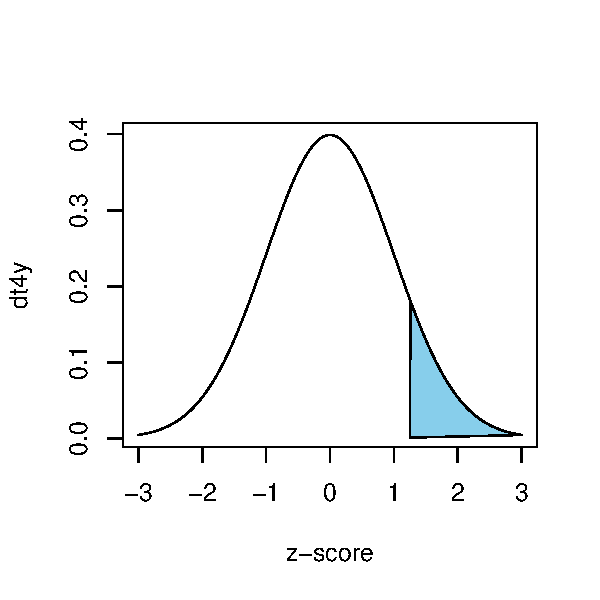
\includegraphics[width=4cm]{figure/LBL8a-1} 


\end{minipage}
\end{frame}

\begin{frame}[fragile]{iClicker Question 6.2}

Recall that if Best Buy sold 100 smart watches last year, the percentage of  watches sold with extended protection plans is expected to be around 20\% give or take 4\%.  What is the chance that the percentage of plans sold with extended warranties is between  $12\% (= 20\% - 2 \times 4\%) \texttt{ and } 28\% (=  20\% + 2 \times 4\%$)?

\begin{enumerate}
\item 99.7\%
\item 95\%
\item 68\%
\item 75\%
\item cannot determine
\end{enumerate}
\end{frame}

\begin{frame}[fragile]{Outline}

% Distribution of the Sample Proportion  

Estimating Proportion

\begin{itemize}
 
\item<1-> Questions Asked About Population Proportion
\end{itemize}
\end{frame}

\begin{frame}[fragile]{Questions Asked}

about the population proportion

\begin{itemize}
\item<1-> The population proportion p are generally unknown and are  estimated from the data.
\item<2-> Suppose we want to estimate the number of students planning to  attend graduate school.
  \begin{enumerate}[1]
   \item<3-> Will the sample proportion equal the population proportion? Yes or  No.
    \item<4-> If not, by how much will it miss?
  \end{enumerate}
\end{itemize}
\end{frame}

\begin{frame}[fragile]{Estimating the population proportion p}

\begin{itemize}
\item<1-> $\hat{p}$ is an estimate of the population proportion, i.e.,
\begin{equation*}
E[ \hat{p} ] = p
\end{equation*}

\item<2-> Our estimate misses it by the standard error of the proportion
\begin{equation*}
SE = \sqrt{ \frac{ \hat{p} (1 - \hat{p})}{n}}
\end{equation*}

\item<3-> Consider our example: $n = 40$ graduating seniors, $X = 6$ plan to  attend graduate school.

\begin{enumerate}[1]
  \item<4-> What is the proportion of graduating seniors planning to attend  graduate school?
  \item<5-> By how much will it miss the true population proportion?
\end{enumerate}
\end{itemize}
\end{frame}

\begin{frame}[fragile]{Estimating the pop. proportion -- Cont'd}

{\small{
\begin{itemize}
\item<1-> $\hat{p} = \frac{X}{n} = \frac{6}{40} = 0.15$

\item<2-> 
\begin{eqnarray*}
SE_{\hat{p}} &=& \sqrt{ \frac{\hat{p} (1 - \hat{p})}{n}} 
= \sqrt{ \frac{.15 \times .85}{40}} \\
&=& 0.056 
\end{eqnarray*}

\item<3-> What if 54 out of 360 students plan to go to graduate school. The  proportion of all students who plan to go to graduate school is  estimated as

\item<4-> $\hat{p} = \frac{54}{360} = 0.15$ with $SE_{\hat{p}} = \sqrt{ \frac{.15 \times .85}{360}} = .0188$

\end{itemize}
}}
\end{frame}

\begin{frame}[fragile]{Estimating the pop. proportion -- Cont'd}

\begin{itemize}
\item<1-> The \textbf{population} proportion $p$ is estimated using the sample proportion $\hat{p}$,  i.e., $E[ \hat{p}] = p$.   

\item<2-> This estimate tends to miss by an amount called the $SE_{\hat{p}}$.

\item<3-> The $SE_{\hat{p}}$ is calculated as 
\begin{equation*}
SE_{\hat{p}} = \sqrt{ \frac{ \hat{p} ( 1 - \hat{p})}{n}}
\end{equation*}

\item<4-> As sample size increases, the $SE_{\hat{p}}$ decreases.
\end{itemize}
\end{frame}

\begin{frame}[fragile]{iClicker Question 8.3}

Which of the following statements is true about the standard error of  the sample proportion?

\begin{enumerate}
\item The standard error increases when sample size  increases.
\item The standard error decreases when sample size  decreases.
\item The increase/decrease of sample size has no effect on  the value of the standard error.
\item The standard error decreases when sample size  increases.
\item None of the previous.
\end{enumerate}
\end{frame}


%!Rnw root = ../../Master.Rnw

\section{STAT 1600 Ch 9 Comparing Two Proportions,  Part 1 Difference in Proportions}

\begin{frame}[fragile]{Statistics and Data Analysis}

STAT 1600 \\ Ch 9 Comparing Two Proportions, \\ Part 1 Difference in Proportions

\end{frame}

\begin{frame}[fragile]{Outline}


Difference Between Independent Proportions  

\begin{itemize}
\item Example and Notation
\item Standard Error of Difference in Sample Proportions
\end{itemize}
\end{frame}

\begin{frame}[fragile]{Change in Student Retention Rate}

\begin{itemize}
\item<1-> Has retention rate at WMU  changing?
\item<2-> A random sample of 200 entering students in 1989 $\Rightarrow$ 74\% were  still enrolled 3 years later.
\item<3-> Another random sample of 200 entering students in 1999 $\Rightarrow$ 66\% were still enrolled 3 years later.
\item<4-> An 8\% change in 3-year retention rate was observed.
\item<5-> The 8\% difference is based on random sampling, and is only an  estimate of the true difference.
\item<6-> What is the likely size of the error of estimation?
\end{itemize}
\end{frame}

\begin{frame}[fragile]{Notation}

A categorical variable with binary responses (`success' and `failure') is of  interest for two independent populations.

\begin{itemize}
\item<1-> Population 1 has proportion $p_1$ of successes.  
\item<2-> Population 2 has proportion $p_2$ of successes.
\item<3-> Sample of size $n_1$  is taken from population 1: $X$ successes observed in the sample with sample proportion $\hat{p_1} = \frac{X}{n_1}$
\item<4-> Sample of size $n_2$  is taken from population 2: $Y$ successes observed in the sample with sample proportion $\hat{p_2} = \frac{Y}{n_2}$
\item<5-> The two samples are independent.
\end{itemize}
\end{frame}

\begin{frame}[fragile]{Standard Error of Difference}

The SE (Standard Error) of the difference in the sample proportions of  two independent samples is

$$SE_{\hat{p_1} - \hat{p_2}} = \sqrt{ (SE_{\hat{p_1}})^2 + (SE_{\hat{p_2}})^2} $$

where

{\small{
$$ SE_{\hat{p_1}} = \sqrt{ \frac{ \hat{p}_1 ( 1 - \hat{p}_1)}{n_1}} $$

$$ SE_{\hat{p_2}} = \sqrt{ \frac{ \hat{p}_2 ( 1 - \hat{p}_2)}{n_2}} $$
}}
\end{frame}

\begin{frame}[fragile]{Change in Student Retention Rate}

{\footnotesize{
\begin{itemize}
\item<1-> For 1989 sample $\hat{p}_1 = 0.74$ give or take (i.e., with a standard error)
$$ SE_{\hat{p_1}} = \sqrt{ \frac{ 0.74 ( 0.26)}{200}} = \sqrt{0.000962} = 0.031 $$

\item<2-> For 1999 sample $\hat{p}_2 = 0.66$ give or take (i.e., with a standard error)
$$ SE_{\hat{p_2}} = \sqrt{ \frac{ 0.66 ( 0.34)}{200}} = \sqrt{0.001122} = 0.033 $$

\item<3-> and hence for the difference in sample proportions.
$$SE_{\hat{p_1} - \hat{p_2}} = \sqrt{ 0.000962 + 0.001122} = 0.0456 $$

\end{itemize}
}}
\end{frame}

\begin{frame}[fragile]{Calculation of the $SE_{\hat{p}_1 - \hat{p}_2}$}

{\footnotesize{
\begin{itemize}
\item<1-> Calculate ($SE_1)^2$, the squared $SE_{\hat{p_1}}$
\begin{equation*}
  (SE_1)^2 =  \frac{ \hat{p}_1 (1 - \hat{p}_1)}{n_1}
\end{equation*}
keeping 6 decimal places to the right of the decimal point.  
\item<2-> Calculate ($SE_2)^2$, the squared $SE_{\hat{p_2}}$
\begin{equation*}
  (SE_2)^2 = \frac{ \hat{p}_2 (1 - \hat{p}_2)}{n_2} 
\end{equation*}
keeping 6 decimal places to the right of the decimal point.  
\item<3-> Calculate $(SE_1)^2 + (SE_2)^2$.
\item<4-> $SE_{\hat{p}_1 - \hat{p}_2} = \sqrt{(SE_1)^2 + (SE_2)^2}$

\end{itemize}
}}
\end{frame}

\begin{frame}[fragile]{Calculation of the $SE_{\hat{p}_1 - \hat{p}_2}$}

Change in Retention Rate Example

\begin{eqnarray*}
(SE_1)^2 &=& \frac{.74 \times .26}{200} = 0.000962 \\
(SE_2)^2 &=& \frac{.66 \times .34}{200} = 0.001122 \\
(SE_1)^2 + (SE_2)^2 &=& 0.000962 + 0.001122 = 0.002084 \\
SE_{ \hat{p}_1 - \hat{p}_2} &=& \sqrt{0.002084} = 0.0456
\end{eqnarray*}
\end{frame}

\begin{frame}[fragile]{Outline}

Confidence Interval for Difference in Proportions  

\begin{itemize}
\item Confidence Interval for Difference in Proportions  
\item iClicker Questions
\end{itemize}

\end{frame}

\begin{frame}[fragile]{Confidence Interval for $\hat{p}_1 - \hat{p}_2$}

{\small{
A 95\% confidence interval for the true difference $p_1 - p_2$ is

$$\hat{p}_1 - \hat{p}_2 \pm 1.96 \times SE_{ \hat{p}_1 - \hat{p}_2}$$

That is 

$$\hat{p}_1 - \hat{p}_2 \pm 1.96 \sqrt{ \frac{\hat{p}_1 (1-\hat{p}_1)}{n_1} + \frac{\hat{p}_2 (1-\hat{p}_2)}{n_2}}$$

\textit{If the interval excludes zero (0), then we say that the difference in sample proportions is statistically significant.} \\ However, If the interval includes 0 then the difference is statistically insignificant.
}}
\end{frame}

\begin{frame}[fragile]{Change in Student Retention Rate}

{\small{
\begin{itemize}
\item<1-> Recall that the standard error of the difference in the sample  proportions is
$$SE_{\hat{p}_1 - \hat{p}_2} = 0.0456$$
\item<2-> So, a 95\% CI (confidence interval) for $p_1 - p_2$ is
$(0.74 - 0.66) \pm 1.96 \times 0.0456 = 0.8 \pm 0.089 \Rightarrow$ (-.009, 0.169) 
\item<3-> If we round it off to (-.01, .17), or, in percentages, (-1\%, 17\%), we say  that the drop in retention rate from 1989 to 1999 is between -1\% and  17\% with 95\% confidence. 
\item<4-> Note: 0\% is contained in this interval and  hence there is still a probability that there might not be a real change in retention rate, just chance variability.
\end{itemize}
}}
\end{frame}

\begin{frame}[fragile]{iClicker Question 9.1}

A 95\% confidence interval was constructed for the difference in the  proportions $p_1 - p_2$ in two independent populations: (-0.08, 0.26).  Which of the following is true?

\begin{enumerate}
\item The difference in the proportions is significant.
\item $p_1$  differs from $p_2$ significantly.
\item The difference in the proportions is insignificant.
\item None of the previous.
\end{enumerate}

\end{frame}

\begin{frame}[fragile]{iClicker Question 9.2}

{\small{
A study of the television viewing preferences of children, each child is  asked if the Sesame Street is the program he or she likes the best  among others. Of 200 girls surveyed, 85 like Sesame Street the best;  of 100 boys surveyed, 30 like Sesame Street the best. A 95\%  confidence interval for the difference in the percentages of children like  the Sesame Street the best between girls and boys is (1.2\%,23.8\%).

\begin{enumerate}
\item Which of the following is true?
\item The two percentages differ significantly.
\item The two percentages do not differ significantly.
\item The two proportions do not differ significantly.
\item None of the previous.
\end{enumerate}
}}
\end{frame}

\begin{frame}[fragile]{Outline}

Statistical Significance  

\end{frame}

\begin{frame}[fragile]{Cooks or Chefs}

\begin{itemize}
\item According to a 2009 occupation survey by the Census Bureau, regular cooks were a separate classification from chefs or head cooks:

\vspace{3mm}

\begin{tabular}{@{} ccccc @{}} \hline
Occupation & Women & Men & Total & \% Women \\ \hline
Cooks & 441 & 762 & 1203 & 37 \\
Chefs & 45  & 245 & 290  & 16 \\ \hline
\end{tabular}

\item The difference in percentage is approximately 21\%.
\item Is the difference in percentages just luck of the draw, or due to something  else besides chance?
\end{itemize}
\end{frame}

\begin{frame}[fragile]{Cooks or Chefs -- Cont'd}

\begin{itemize}
\item If chance was at work, how likely we get a difference in proportions of  0.21?
\item The chance of this occurs is small $\Rightarrow < 0.0001$. That is, less than 1 in 10,000.  This chance of getting 0.21 by chance is called a P-value.
\item But how do we know that this P-value is less than 0.0001?
\end{itemize}
\end{frame}

\begin{frame}[fragile]{Cooks or Chefs -- Cont'd}

{\small{
\begin{itemize}
\item The SE for the difference in proportion is
$$ SE_{\hat{p}_1 - \hat{p}_2} = \sqrt{ \frac{ .37 \cdot .63}{1203} + \frac{ .16 \cdot .84}{290} } = 0.026 $$ 
\item And hence the chance to get a difference beyond $\pm 0.078$ (= 3SE ) is 0.003  (= 1 - .997 by the empirical rule), or 3 in 1,000.
\item Similarly, the chance to get a difference beyond $\pm 0.104$ (= 4SE ) is $0.00006 < 0.0001$, or less than 1 in 10,000.
\item Now, in our example, a difference of 0.21 is beyond 8 SE. This cannot be  just chance variability.  Something else is at work.
\item Note: the probability of 0.00006 above was obtained by computer.
\end{itemize}
}}
\end{frame}

\begin{frame}[fragile]{Statistical Significance, The P-Value}

The general rule for P-value for the difference:

\begin{itemize}
\item If P-value $\le .05$, the difference is \textbf{statistically significant}.  (difference is at least 1.96SE in absolute value)
\item If P-value $\le .01$, the difference is called \textbf{highly significant}.  (difference is at least 2.58SE in absolute value)
\item If P-value $> .05$, the difference is \textbf{insignificant}. (difference is less  than 1.96SE in absolute value)
\end{itemize}
\end{frame}

\begin{frame}[fragile]{iClicker Question 9.3}

A 95\% confidence interval was constructed for difference in the proportions $p_1 - p_2$ in two independent populations: (-0.04, 0.16). Which of the following is true?

\begin{enumerate}
\item The p-value $\le 0.05$, the difference is statistically significant.
\item The p-value $\le 0.01$, the difference is called highly significant.
\item The p-value $> 0.05$, the difference is insignificant.
\item None of the above.
\end{enumerate}
\end{frame}


%!Rnw root = ../../Master.Rnw

\section{Stat1600 Ch 9.3.2 Comparing Two  Proportions, Part 2 Risk Ratio}

\begin{frame}[fragile]{Statistics and Data Analysis}

Stat1600 \\ Ch 9.3.2 Comparing Two  Proportions, \\ Part 2 Risk Ratio

\end{frame}

\begin{frame}[fragile]{Outline}

Risk Ratio  

\begin{itemize}
\item Risk Ratio
\item iClicker Questions
\end{itemize}

\end{frame}

\begin{frame}[fragile]{Hepatitis E Vaccine}

From the study `Safety and Efficacy of a Recombinant Hepatitis E  Vaccine' by Shrestha et al. in the New England Journal of Medicine in  March 2007 (Vol. 356 No. 9), the results were

\begin{tabular}{@{} cccc @{}} \hline
     & \multicolumn{2}{c}{Hepatitis E} \\
     & Yes & No & Total \\ \hline
Vaccine & 3 & 895 & 898 \\
Placebo & 66 & 830 & 896 \\ \hline
\end{tabular}

The vaccine efficacy, as reported in the article, was 95.5\% with a 95\%  confidence interval of \\ (85.6\%, 98.6\%). \\
How?

\end{frame}

\begin{frame}[fragile]{Risk ratio}

{\small{
Consider:
\vspace{2mm}

\begin{tabular}{@{} cccc @{}} \hline
     & \multicolumn{2}{c}{Disease} \\
     & Yes & No & Total \\ \hline
Exposure & a & b & a + b \\
No exposure & c & d & c + d \\ \hline
\end{tabular}

where Exposure = Exposure to treatment (i.e., Vaccine in this example).

\vspace{2mm}

The \textit{risk ratio} (or relative risk) is

\begin{equation*}
RR = \frac{ P[ Disease, exposure]}{ P[ Disease, No exposure]} = \frac{ \frac{a}{a+b}}{ \frac{c}{c+d}} 
\end{equation*}

and the \textit{efficacy} of the exposure is (1 - risk ratio) \\ if \texttt{risk ratio} $ \le 1$. 

}}
\end{frame}

\begin{frame}[fragile]{Hepatitis E Vaccine Eg., Cont'd}

\begin{equation*}
RR = \frac{ \frac{3}{898}}{ \frac{66}{896}} = 0.045 \texttt{ or } 4.5\%
\end{equation*}

\vspace{3mm}

That is, getting the vaccine reduces your risk to only 4.5\% of the  original. The efficacy of the vaccine is 95.5\% (= 100\% - 4.5\%)

\end{frame}

\begin{frame}[fragile]{Calculating a 95\% CI for RR}

{\small{
\begin{enumerate}
\item<1-> Calculate a 95\% confidence interval for ln(RR):
  \begin{enumerate}
  \item<2-> calculate ln(RR)
  \item<3-> calculate
  \begin{equation*}
    SE_{ln(RR)} = \sqrt{\frac{1}{a} + \frac{1}{c} - \frac{1}{a+b} - \frac{1}{c+d}}
  \end{equation*}
  \item<4-> calculate 95\% CI for ln(RR)
  \begin{equation*}
    (ln(RR) - 1.96 SE, ln(RR) + 1.96 SE )
  \end{equation*}
  \end{enumerate}
\item<5-> A 95\% confidence interval for RR is
\begin{equation*}
    (e^{ln(RR) - 1.96 SE}, e^{ln(RR) + 1.96 SE} )
  \end{equation*}
  
\item<6-> and RR is statistical significant if the interval excludes one (1).
\end{enumerate}
}}
\end{frame}

\begin{frame}[fragile]{Hepatits E Vaccine Example, Cont'd}

{\small{
\begin{enumerate}
\item<1-> Calculate a 95\% confidence interval for ln(RR):
  \begin{enumerate}
  \item<2-> calculate ln(RR) = ln(.045) = -3.101
  \item<3-> calculate
  \begin{eqnarray*}
    SE_{ln(RR)} &=& \sqrt{\frac{1}{3} + \frac{1}{66} - \frac{1}{3+898} - \frac{1}{66+896}}  \\
    &=& \sqrt{.3462} \\
    &=& 0.5884 
  \end{eqnarray*}
  \item<4-> calculate 95\% CI for ln(RR)
  \begin{eqnarray*}
    CI &=& (-3.101-1.96 \cdot .5884, -3.101+1.96 \cdot .5884) \\
    &=& (-4.254, -1.948)
  \end{eqnarray*}
  \end{enumerate}
\end{enumerate}  
}}
\end{frame}

\begin{frame}[fragile]{Hepatits E Vaccine Example, Cont'd}

\begin{enumerate}
\item<1-> A 95\% confidence interval for RR is
\begin{equation*}
    (e^{-4.254}, e^{-1.948} ) = (.014, .143)
  \end{equation*}
  
\item<2-> That is, with 95\% confidence, the relative risk of getting hepatitis with the vaccine is only 1.4\% to 14.3\% of placebo. In other words, the vaccine reduces your risk by as low as 85.7\% (=100\% - 14.3\%) or as high as 98.6\% (= 100\% - 1.4\%).
\end{enumerate}

\end{frame}

\begin{frame}[fragile]{iClicker Question 9.2.1}

In an observational study, a sample of 10000 smokers was taken, 50  were found to have lung cancer. Another sample of 10000 non-smokers was taken, only 2 have lung cancer. What is the relative  risk of having lung cancer for smokers versus non-smokers?

\begin{enumerate}
  \item 50
  \item 2
  \item 25  
  \item 100
  \item cannot determine
\end{enumerate}
\end{frame}

\begin{frame}[fragile]{iClicker Question 9.2.2}

In an observational study, a sample of 10000 smokers was taken, 50  were found to have lung cancer. Another sample of 10000 non-smokers was taken, only 2 have lung cancer. A 95\% confidence  interval for the relative risk of having lung cancer for smokers versus  smokers is (6.1, 102.5). Which of the following is true?

\begin{enumerate}
\item The proportion of smokers having lung cancer is  significantly different than that of non-smokers.
\item There is no difference between the two proportions.
\item cannot determine
\end{enumerate}
\end{frame}


%!Rnw root = ../../Master.Rnw

\section{Stat1600 Ch 9.3.3 Comparing Two  Proportions, Part 3 Odds Ratio}

\begin{frame}[fragile]{Statistics and Data Analysis}

Stat 1600 \\ Ch 9.3.3 Comparing Two  Proportions, Part 3 Odds Ratio

\end{frame}

\begin{frame}[fragile]{Outline}

\begin{itemize}
\item Odds Ratio
\item iClicker Questions
\end{itemize}
\end{frame}

\begin{frame}[fragile]{Odds}

The odds that an event occurs is

{\small{
\begin{equation*}
Odds = \frac{ \texttt{Probability that an event occurs}}{ \texttt{Probability that event does not occur}} = \frac{p}{1 - p}
\end{equation*}
}}

\begin{table}[ht]
\centering
\begin{tabular}{@{} cc @{}} \hline
Probability & Odds \\
0.10 & $\frac{1}{9} = 0.11$ \\
0.20 & $\frac{1}{4} = 0.25$ \\
0.50 & $\frac{1}{1} = 1.00$ \\
0.80 & $\frac{4}{1} = 4.00$ \\
0.90 & $\frac{9}{1} = 9.00$ \\
\end{tabular}
\end{table}
\end{frame}

\begin{frame}[fragile]{iClicker Question 15.1}

{\small{
A clinical trial was conducted to study the efficacy of a new drug  intended to lower the LDL (low-density lipoprotein, a.k.a., bad  cholesterol). All study subjects showed a high LDL level at the baseline.  Of the 100 treated subjects, 80 of them showed reduction to normal  LDL level two weeks after treatment. What is the odds that a treated  subject was having a reduction in LDL to normal level after two weeks?

\begin{enumerate}
\item 0.25
\item 4
\item 80
\item 20
\item cannot determine
\end{enumerate}
}}
\end{frame}

\begin{frame}[fragile]{Outline}

\begin{itemize}
\item Odds Ratio
\item iClicker Questions
\end{itemize}
\end{frame}


% \begin{frame}[fragile]{Hepatitis E Vaccine Eg., Cont'd}
% 
% \begin{equation*}
% RR = \frac{ \frac{3}{898}}{ \frac{66}{896}} = 0.045 \texttt{ or } 4.5\%
% \end{equation*}
% 
% \vspace{3mm}
% 
% That is, getting the vaccine reduces your risk to only 4.5\% of the  original. The efficacy of the vaccine is 95.5\% (= 100\% - 4.5\%)
% 
% \end{frame}
% 
% \begin{frame}[fragile]{Calculating a 95\% CI for RR}
% 
% {\small{
% \begin{enumerate}
% \item<1-> Calculate a 95\% confidence interval for ln(RR):
%   \begin{enumerate}
%   \item<2-> calculate ln(RR)
%   \item<3-> calculate
%   \begin{equation*}
%     SE_{ln(RR)} = \sqrt{\frac{1}{a} + \frac{1}{c} - \frac{1}{a+b} - \frac{1}{c+d}}
%   \end{equation*}
%   \item<4-> calculate 95\% CI for ln(RR)
%   \begin{equation*}
%     (ln(RR) - 1.96 SE, ln(RR) + 1.96 SE )
%   \end{equation*}
%   \end{enumerate}
% \item<5-> A 95\% confidence interval for RR is
% \begin{equation*}
%     (e^{ln(RR) - 1.96 SE}, e^{ln(RR) + 1.96 SE} )
%   \end{equation*}
%   
% \item<6-> and RR is statistical significant if the interval excludes one (1).
% \end{enumerate}
% }}
% \end{frame}
% 
% \begin{frame}[fragile]{Hepatits E Vaccine Example, Cont'd}
% 
% {\small{
% \begin{enumerate}
% \item<1-> Calculate a 95\% confidence interval for ln(RR):
%   \begin{enumerate}
%   \item<2-> calculate ln(RR) = ln(.045) = -3.101
%   \item<3-> calculate
%   \begin{eqnarray*}
%     SE_{ln(RR)} &=& \sqrt{\frac{1}{3} + \frac{1}{66} - \frac{1}{3+898} - \frac{1}{66+896}}  \\
%     &=& \sqrt{.3462} \\
%     &=& 0.5884 
%   \end{eqnarray*}
%   \item<4-> calculate 95\% CI for ln(RR)
%   \begin{eqnarray*}
%     CI &=& (-3.101-1.96 \cdot .5884, -3.101+1.96 \cdot .5884) \\
%     &=& (-4.254, -1.948)
%   \end{eqnarray*}
%   \end{enumerate}
% \end{enumerate}  
% }}
% \end{frame}
% 
% \begin{frame}[fragile]{Hepatits E Vaccine Example, Cont'd}
% 
% \begin{enumerate}
% \item<1-> A 95\% confidence interval for RR is
% \begin{equation*}
%     (e^{-4.254}, e^{-1.948} ) = (.014, .143)
%   \end{equation*}
%   
% \item<2-> That is, with 95\% confidence, the relative risk of getting hepatitis with the vaccine is only 1.4\% to 14.3\% of placebo. In other words, the vaccine reduces your risk by as low as 85.7\% (=100\% - 14.3\%) or as high as 98.6\% (= 100\% - 1.4\%).
% \end{enumerate}
% 
% \end{frame}
% 
% \begin{frame}[fragile]{iClicker Question 9.2.1}
% 
% In an observational study, a sample of 10000 smokers was taken, 50  were found to have lung cancer. Another sample of 10000 non-smokers was taken, only 2 have lung cancer. What is the relative  risk of having lung cancer for smokers versus non-smokers?
% 
% \begin{enumerate}
%   \item 50
%   \item 2
%   \item 25  
%   \item 100
%   \item cannot determine
% \end{enumerate}
% \end{frame}
% 
% \begin{frame}[fragile]{iClicker Question 9.2.2}
% 
% In an observational study, a sample of 10000 smokers was taken, 50  were found to have lung cancer. Another sample of 10000 non-smokers was taken, only 2 have lung cancer. A 95\% confidence  interval for the relative risk of having lung cancer for smokers versus  smokers is (6.1, 102.5). Which of the following is true?
% 
% \begin{enumerate}
% \item The proportion of smokers having lung cancer is  significantly different than that of non-smokers.
% \item There is no difference between the two proportions.
% \item cannot determine
% \end{enumerate}
% \end{frame}




% 
% 
% <<Sec2, child="sections/section2/section2.Rnw",eval=TRUE>>=  
% @
% 
% <<Sec3, child="sections/section3/section3.Rnw",eval=TRUE>>=   
% @
% 
% <<Sec4, child="sections/section4/section4.Rnw",eval=TRUE>>=  
% @
% 
% <<label=LBLrn, results="asis", echo=FALSE>>=
%   system('mv Master.pdf ch1.pdf')
% @

% \printbibliography
%\bibliographystyle{plain}
%\bibliography{chapters/mybibliography}   % name your BibTeX data base

% \section{Index}

% \printindex

\end{document}
